 
 
 

\chapter{Infinite Series of Numbers and Infinite Products }\label{ch5}
In this chapter, we discuss infinite series of numbers and infinite products.
 
 
\section{Limit Superior and Limit Inferior}\label{sec5.1}
In Chapter \ref{ch1}, we have seen that a bounded sequence might not be convergent. In this section, we will   discuss the concepts called limit inferiors and limit superiors, which characterize the limits of subsequences of a sequence. 

First we extend the definitions of supremum and infimum as follows. 
\begin{highlight}{Extensions of Infmum and Supremum}
\begin{enumerate}[1.]
\item  If a nonempty set $S$ is not bounded below, we write $\inf S=-\infty$.
\item If a nonempty set $S$ is not bounded above, we write $\sup S=\infty$.

\item $\inf\{-\infty\}=-\infty, \inf\{\infty\}=\infty$.
\item $\sup\{-\infty\}=-\infty, \sup\{\infty\}=\infty$.
\end{enumerate}
\end{highlight}
The definition of limits are also extended to include $-\infty$ and $\infty$ as limits.
 
\begin{theorem}[label=230603_2]{}
Let $\{a_n\}$ be a sequence of real numbers.
\begin{enumerate}[1.]
\item The sequence $\{a_n\}$ is  not bounded above if and only if there is a strictly increasing subsequence $\{a_{n_k}\} $ such that $\di\lim_{k\to\infty}a_{n_k}=\infty$.
\item The sequence $\{a_n\}$ is  not bounded below if and only if there is a strictly decreasing subsequence $\{a_{n_k}\} $ such that $\di\lim_{k\to\infty}a_{n_k}=-\infty$.

\end{enumerate}
\end{theorem}
\begin{myproof}
{Proof}
It is sufficient to prove the first statement. If there is a subsequence $\{a_{n_k}\}$ of $\{a_n\}$ such that $\di\lim_{k\to\infty}a_{n_k}=\infty$, it is obvious that $\{a_n\}$ is not bounded above. 

Conversely,
 given that $\{a_n\}$ is not bounded above, we want to construct a strictly increasing subsequence $\{a_{n_k}\}$  such that $\di\lim_{k\to\infty}a_{n_k}=\infty$.  Let $n_1=1$. 
Since $\{a_n\}$ is not bounded above, there is a $n_2 >1$ such that $a_{n_2}\geq a_{n_1}+1$. Assume we have found $n_1, n_2, \ldots, n_{k-1}$, such that
\[n_1<n_2<\cdots<n_{k-1},\]and
\[a_{n_{j+1}}\geq a_{n_{j}}+1, \hspace{1cm}\text{for all}\;1\leq j\leq k-2.\]Since $\{a_n\}$ is not bounded above, there is an $n_k>n_{k-1}$ such that $a_{n_k}\geq a_{n_{k-1}}+1$. This constructs a strictly increasing sequence $\{a_{n_k}\}$ inductively which satisfies
\[ a_{n_{k+1}}\geq a_{n_{k}}+1, \hspace{1cm}\text{for all}\;k\in\mathbb{Z}^+.\] From this, we find that
\[a_{n_k}\geq a_{n_1}+k-1.\]  Therefore,  $\di\lim_{k\to\infty}a_{n_k}=\infty$.



\end{myproof}
Associated with a given sequence $\{a_n\}$, we can define two sequences $\{b_n\}$ and $\{c_n\}$.
\begin{definition}{}
Given a sequence $\{a_n\}$, we can define two sequences $\{b_n\}$ and $\{c_n\}$ as follows. For each positive integer $n$,  
\[b_n=\inf_{k\geq n}a_k=\inf\{a_k\,|\,k\geq n\},\hspace{1cm}c_n=\sup_{k\geq n}a_k=\sup\{a_k\,|\,k\geq n\}.\]

\end{definition}



\begin{example}[label=ex230226_1]{}
For the sequence $\{a_n\}$ with $a_n=\di\frac{1}{n}$,
\[b_n=0,\hspace{1cm} c_n=\frac{1}{n}\hspace{1cm}\text{for all}\;n\geq 1.\]

\end{example}

\begin{example}[label=ex230226_2]{}
For the sequence $\{a_n\}$ with $a_n=n$,
\[b_n=n,\hspace{1cm} c_n=\infty\hspace{1cm}\text{for all}\;n\geq 1.\]

\end{example}

\begin{example}[label=ex230226_3]{}
For the sequence $\{a_n\}$ with $a_n=(-1)^n$,
\[b_n=-1,\hspace{1cm} c_n=1\hspace{1cm}\text{for all}\;n\geq 1.\]

\end{example}
The following are obvious from the definitions and Theorem \ref{230603_2}.
\begin{proposition}[label=230603_1]{}
Given that $\{a_n\}$ is a sequence of real numbers, for each $n\in\mathbb{Z}^+$, let $\di b_n=\inf_{k\geq n}a_k$ and $\di c_n=\sup_{k\geq n}a_k$.  
\begin{enumerate}[1.]
\item For any positive integer $n$,  $b_n\leq a_n\leq c_n$.
\item  For any positive integer $n$,  $b_n$ cannot be $\infty$, $c_n$ cannot be $-\infty$.
\item $\{a_n\}$ is not bounded below if and only    $b_n=-\infty$ for all $n\geq 1$.
\item $\{a_n\}$ is not bounded above if and only if   $c_n=\infty$ for all $n\geq 1$.
 
\item $\{b_n\}$ is an increasing sequence.
\item $\{c_n\}$ is a decreasing sequence.   
\end{enumerate}
\end{proposition}

 

Since $\{b_n\}$ is an increasing sequence, $\di\lim_{n\to \infty}b_n=\sup\{b_n\}$ in the general sense.  Similarly, $\di\lim_{n\to \infty}c_n=\inf\{c_n\}$. 
\begin{definition}{Limit Inferior and Limit Superior}
Let $\{a_n\}$ be a sequence of real numbers.
\begin{enumerate}
[1.]\item The limit inferior or limit infimum of $\{a_n\}$, denoted by $\di\liminf_{n\to\infty}a_n$ or $\di\varliminf_{n\to\infty}a_n$, is defined as
\[\liminf_{n\to\infty}a_n=\lim_{n\to \infty}b_n=\sup_{n\geq 1}\inf_{k\geq n}a_k.\]
\item The limit superior or limit supremum of $\{a_n\}$, denoted by $\di\limsup_{n\to\infty}a_n$ or $\di\varlimsup_{n\to\infty}a_n$, is defined as
\[\limsup_{n\to\infty}a_n=\lim_{n\to \infty} c_n=\inf_{n\geq 1}\sup_{k\geq n}a_k.\]
\end{enumerate}
\end{definition}


Notice that using extended definitions of infimum and supremum, the limit infimum and limit supremum of a sequence always exist, either as a finite number, or $\pm \infty$.

 
\begin{example}{}
\begin{enumerate}[1.]
\item
For the sequence $\{a_n\}$ with $a_n=\di\frac{1}{n}$ defined in Example \ref{ex230226_1},
\[\liminf_{n\to\infty}a_n=0,\hspace{1cm} \limsup_{n\to\infty}a_n=0.\]
\item
For the sequence $\{a_n\}$ with $a_n=n$ defined in Example \ref{ex230226_2},
\[\liminf_{n\to\infty}a_n=\infty, \hspace{1cm} \limsup_{n\to\infty}a_n=\infty.\]
\item
For the sequence $\{a_n\}$ with $a_n=(-1)^n$ defined in Example \ref{ex230226_3},
\[\liminf_{n\to\infty}a_n=-1,\hspace{1cm} \limsup_{n\to\infty}a_n=1.\]
\end{enumerate}
\end{example}
The following are obvious.
\begin{highlight}{}
\begin{enumerate}[1.]\item
$\di \liminf_{n\to\infty}(-a_n)=-\limsup_{n\to\infty}a_n$
\item $\di\limsup_{n\to\infty}(-a_n)=-\liminf_{n\to\infty}a_n$.
\end{enumerate}
\end{highlight}
Since \[b_n\leq c_n\hspace{1cm}\text{for all}\;n\in\mathbb{Z}^+,\]we obtain the following immediately.
\begin{proposition}[label=230227_21]{}
For any sequence $\{a_n\}$,
\[\liminf_{n\to \infty}a_n\leq \limsup_{n\to\infty}a_n.\]
\end{proposition}


We also have the following comparison theorem.
\begin{proposition}{}
Let $\{u_n\}$ and $\{v_n\}$ be sequences of real numbers. If $u_n\leq v_n$ for all positive integers $n$, then
\[\liminf_{n\to\infty}u_n\leq\liminf_{n\to \infty}v_n\hspace{1cm}\limsup_{n\to\infty}u_n\leq\limsup_{n\to \infty}v_n.\]
\end{proposition}



\begin{example}{}Find $\di\liminf_{n\to\infty}a_n$ and $\di \limsup_{n\to \infty}a_n$ for the sequence $\{a_n\}$   defined by
\[a_n=(-1)^n\left(1+\frac{1}{n}\right).\]

\end{example}
\begin{solution}{Solution}
Notice that for any $n\geq 1$,
\[
a_{2n-1}=-1-\frac{1}{2n-1},\hspace{1cm}a_{2n}=1+\frac{ 1}{2n}.
\] \bs We observe that
\[a_1<a_3<\cdots<-1<1<\cdots<a_4<a_2.\]The sequence $\di\{a_{2n-1}\}$ increases to $-1$, while the sequence $\{a_{2n}\}$ decreases to 1. 
Therefore,
\[b_{2n}=b_{2n+1}=-1-\frac{1}{2n+1},\hspace{1cm}c_{2n-1}=c_{2n}=1+\frac{1}{2n}.\]
It follows that
\[\liminf_{n\to\infty}a_n=\lim_{n\to\infty}b_n=-1,\hspace{1cm}
\limsup_{n\to\infty}a_n=\lim_{n\to\infty} c_n= 1.\]
\end{solution}

\begin{example}{}Let $\{a_n\}$ be the sequence defined by
$a_n=(-1)^nn$.
Find $\di\liminf_{n\to\infty}a_n$ and $\di \limsup_{n\to \infty}a_n$.
\end{example}
\begin{solution}{Solution}
For any $n\geq 1$,
\[
a_{2n-1}=-(2n-1),\hspace{1cm}a_{2n}=2n.
\]  The sequence
$\{a_n\}$ is not bounded below nor bounded above. Therefore,
\[b_n=-\infty,\hspace{1cm}c_n=\infty.\]
It follows that
\[\liminf_{n\to\infty}a_n= -\infty,\hspace{1cm}
 \limsup_{n\to\infty}a_n=\infty.\]
\end{solution}


For a monotoic sequence, it is easy to find its limit inferior and limit superior.
\begin{theorem}{}
Let $\{a_n\}$ be a monotonic sequence.
\begin{enumerate}[1.]
\item If $\{a_n\}$ is increasing, then $b_n=a_n$ and $c_n=\sup\{a_n\}$. Therefore,
\[\liminf_{n\to\infty}a_n=\limsup_{n\to\infty}a_n=\lim_{n\to\infty}a_n=\sup\{a_n\}.\]
\item  If $\{a_n\}$ is decreasing, then $b_n=\inf\{a_n\}$ and $c_n=a_n$. Therefore,
\[\liminf_{n\to\infty}a_n=\limsup_{n\to\infty}a_n=\lim_{n\to\infty}a_n=\inf\{a_n\}.\]

\end{enumerate}
\end{theorem}
In other words, for monotonic sequence, the limit inferior, limit superior, and the limit are all the same.

In fact, if a sequence $\{a_n\}$ has a finite limit, then its limit inferior, limit superior and limit are all the same.
\begin{theorem}{}
Let $\{a_n\}$ be a sequence, and let $a$ be a finite number. Then the following two statements are equivalent.
\begin{enumerate}[(a)]
\item   $\di\lim_{n\to\infty}a_n=a$.
\item $\di \liminf_{n\to \infty}a_n=\limsup_{n\to \infty}a_n=a$.
 \end{enumerate}
\end{theorem}
\begin{myproof}
{Proof}
For a positive integer $n$, define
$\di b_n=\inf_{k\geq n}a_k$, $c_n=\sup_{k\geq n}a_n$.
Then
\[\liminf_{n\to \infty}a_n=\lim_{n\to\infty}b_n,\hspace{1cm}\limsup_{n\to \infty}a_n=\lim_{n\to\infty}c_n.\]
By definition,
\[b_n\leq a_n\leq c_n.\]
Hence, (b) implies (a) follows from squeeze theorem.
\bp
Now we prove that (a) implies (b). Given $\varepsilon>0$, since $\di\lim_{n\to\infty}a_n=a$, there is a positive integer $N$ such that for all $n\geq N$, 
\[a-\frac{\varepsilon}{2}<a_n<a+\frac{\varepsilon}{2}.\]
Hence, for all $n\geq N$,
\[ a-\frac{\varepsilon}{2}\leq b_n\leq a+\frac{\varepsilon}{2}\hspace{1cm}\text{and}\hspace{1cm}a-\frac{\varepsilon}{2}\leq c_n\leq a+\frac{\varepsilon}{2}.\]
These prove that for all $n\geq N$,
\[|b_n-a|<\varepsilon\hspace{1cm}\text{and}\hspace{1cm}|c_n-a|<\varepsilon.\]
Thus,
\[\liminf_{n\to \infty}a_n=\limsup_{n\to \infty}a_n=a.\]
\end{myproof}

Hence, we are left to consider sequences which does not have a finite limit.
 Let us first characterize when  the limit inferior and the limit superior of a sequence  can be $-\infty$ or $\infty$. 
\begin{theorem}[label=230226_1]{}
Let $\{a_n\}$ be a sequence of real numbers. Then the following three statements are equivalent.
\begin{enumerate}[(a)]
\item $\di\limsup_{n\to\infty}a_n=\infty$.
\item $\{a_n\}$ is not bounded above.
\item  There is a strictly increasing subsequence $\{a_{n_k}\}$ such that $\di\lim_{k\to\infty}a_{n_k}=\infty$.


\end{enumerate}
\end{theorem}

\begin{myproof}
{Proof}
Notice that $\di\limsup_{n\to\infty}a_n= \lim_{n\to \infty}c_n$, where $\di c_n=\sup_{k\geq n}a_k$. Since $\{c_n\}$ is a decreasing sequence, $\di\lim_{n\to \infty}c_n=\infty$ if and only if $c_n=\infty$ for all $n\geq 1$. Hence, this theorem  follows  from Theorem \ref{230603_2} and Proposition \ref{230603_1}. 
 


\end{myproof}
 
The limit inferior  version of Theorem \ref{230226_1} is straightforward.
\begin{theorem}[label=230226_2]{}
Let $\{a_n\}$ be a sequence of real numbers. Then the following three statements are equivalent.
\begin{enumerate}[(a)]
\item $\di\liminf_{n\to\infty}a_n=-\infty$.
\item $\{a_n\}$ is not bounded below.
\item  There is a strictly decreasing subsequence $\{a_{n_k}\}$ such that $\di\lim_{k\to\infty}a_{n_k}=-\infty$.


\end{enumerate}
\end{theorem}

What is more nontrivial is when  limit superior is $-\infty$, or limit inferior is $\infty$.

\begin{theorem}[label=230226_3]{}
Let $\{a_n\}$ be a sequence of real numbers.
\begin{enumerate}[1.]
\item
$\di\limsup_{n\to\infty}a_n=-\infty$ if and only if   $\di\lim_{n\to\infty}a_n=-\infty$.
\item $\di\liminf_{n\to\infty}a_n= \infty$ if and only if  $\di\lim_{n\to\infty}a_n= \infty$.
\end{enumerate}
\end{theorem}

\begin{myproof}{Proof}Notice that if $\di\limsup_{n\to\infty}a_n=-\infty$, we must have $\di\liminf_{n\to\infty}a_n=-\infty$. Similarly, if $\di\liminf_{n\to\infty}a_n= \infty$, it is necessary that $\di\limsup_{n\to\infty}a_n= \infty$.

It is enough for us to prove the second statement. 
Let $b_n=\di\inf_{k\geq n }a_k$. Notice that $b_n\leq a_n$. If 
 $\di\liminf_{n\to\infty}a_n= \lim_{n\to\infty}b_n=\infty$, we must have
$\di\lim_{n\to\infty}a_n=\infty$.  Conversely, assume that $\di\lim_{n\to\infty}a_n=\infty$. Given $M>0$, there is a positive integer $N$ such that 
\[a_n\geq M\hspace{1cm}\text{for all}\;n\geq M.\]
This implies that
\[b_n\geq M\hspace{1cm}\text{for all}\;n\geq M.\] Hence, $\di\liminf_{n\to\infty} a_n=\lim_{n\to\infty}b_n=\infty$.
 

\end{myproof}


\begin{example}{}
Consider the sequence $\{a_n\}$ with $a_n=n+(-1)^{n}$. The first few terms are given by
$0, 3, 2, 5, 4, 7, \ldots$.
This sequence is neither increasing nor decreasing. For any $n\geq 1$,
\[b_{2n-1}=b_{2n}=a_{2n-1}=2n-2,\]
while $c_n=\infty$ for all $n\in\mathbb{Z}^+$. Therefore, \[\liminf_{n\to\infty}a_n=\lim_{n\to\infty}b_n=\infty.\]
\end{example}

Combining Theorem \ref{230226_1}, Theorem \ref{230226_2} and Theorem \ref{230226_3}, we can summarize the cases where the limit inferior or the limit superior is $-\infty$ or $\infty$.
\begin{highlight}{Infinities as Limit Superior or Limit Inferior}
Let $\{a_n\}$ be a sequence of real numbers.
\begin{enumerate}[1.]
\item $\di\liminf_{n\to\infty}a_n=\limsup_{n\to\infty}a_n=-\infty$ if and only if $\di\lim_{n\to\infty}a_n=-\infty$. In this case, $\{a_n\}$ is bounded above, not bounded below.
\item $\di\liminf_{n\to\infty}a_n=\limsup_{n\to\infty}a_n= \infty$ if and only if $\di\lim_{n\to\infty}a_n= \infty$. In this case, $\{a_n\}$ is bounded below, not bounded above.
\item $\di\liminf_{n\to\infty}a_n=-\infty$ and $\di\limsup_{n\to\infty}a_n= \infty$ if and only if $\{a_n\}$ is not bounded above nor bounded below.
\item  $-\infty<\di\liminf_{n\to\infty}a_n<\infty$ and $\di\limsup_{n\to\infty}a_n= \infty$ if and only if $\{a_n\}$ is bounded below but not bounded above.
\item $\di\liminf_{n\to\infty}a_n=-\infty$ and $\di -\infty<\limsup_{n\to\infty}a_n< \infty$ if and only if $\{a_n\}$ is bounded above but not bounded below.
\end{enumerate}
\end{highlight}
 
The following gives a relation of limit inferior and limit superior with limits of subsequences.
\begin{theorem}[label=230226_8]{}
Let $\{a_n\}$ be sequence with \[ \liminf_{n\to\infty}a_n=b\quad \text{and}\quad \limsup_{n\to\infty}a_n=c.\] If $\{a_{n_k}\}$ is a subsequence of $\{a_n\}$ that converges to a number $\ell$, then
\[b\leq \ell \leq c.\] Here $b$ and $c$ can be $\pm\infty$.
\end{theorem}
\begin{myproof}{Proof}For every positive integer $n$, let 
\[b_n=\inf_{k\geq n}a_k,\hspace{1cm}c_n=\sup_{k\geq n}a_n.\]
Then
\[b=\lim_{n\to\infty}b_n,\hspace{1cm}c =\lim_{n\to\infty} c_n.\]Given a subsequence $\{a_{n_k}\}$, 
$\{b_{n_k}\}$ and $\{c_{n_k}\}$ are subsequences of the monotonic sequences $\{b_n\}$ and $\{c_n\}$. Hence, we  have
\[\lim_{k\to\infty}b_{n_k}=b,\hspace{1cm}\lim_{k\to\infty}c_{n_k}=c,\]which still holds in the extended sense.
Since \[b_{n_k}\leq a_{n_k}\leq c_{n_k}\hspace{1cm}\text{for all}\;k\in\mathbb{Z}^+,\]we find that
\[b\leq\ell\leq c.\]
\end{myproof}

Now we turn to the case of finite limit superior and finite limit inferior.
We have the following equivalence.
\begin{theorem}[label=230226_5]{}
Let $\{a_n\}$ be a sequence of real numbers. Then  the following two statements are equivalent.
\begin{enumerate}[(a)]
\item $\di\limsup_{n\to\infty}a_n=c$ is finite.
\item Given $\varepsilon>0$, \begin{enumerate}[(i)]\item
there exists a positive integer $N$ such that for all $n\geq N$, $a_n<c+\varepsilon$; and 
\item for every 
  positive integer $N$, there exists an integer $n\geq N$, such that $a_n>c-\varepsilon$.
 \end{enumerate}\end{enumerate}
\end{theorem}

\begin{myproof}{Proof}
For a positive integer $n$, define $\di c_n=\sup_{k\geq n}a_n$, so that $\di\limsup_{n\to\infty}a_n=\lim_{n\to\infty}c_n$.

Let us first prove that (a) implies (b). Given $\varepsilon>0$, since $\di\lim_{n\to\infty}c_n=c$,  there is a positive integer $N$ such that for all $n\geq N$, $
\di |c_n-c|<\varepsilon$.
If $n\geq N$, we find that
\[a_n\leq\sup_{k\geq n}a_k=c_n<c+\varepsilon.\]This proves (b)(i). Now given $\varepsilon>0$,  there is a positive integer $N_0$ such that $c-\varepsilon<c_n<c+\varepsilon$ for all $n\geq N_0$.
For any positive integer $N$, let $N'=\max\{N, N_0\}$. Then $N'\geq N_0$. Hence,
\[ \sup_{k\geq N'}a_k=c_{N'}>c-\varepsilon.\]This implies that $c-\varepsilon$ is not an upper bound of $\{a_k\,|\,k\geq N'\}$. Therefore, there is an $n\geq N'\geq N$ such that $a_n>c-\varepsilon$. This proves (b)(ii).

Now we prove (b) implies (a).  Given $\varepsilon>0$, (b)(i) implies that there is a positive integer $N$ such that for all $n\geq N$, 
\[a_n<c+\frac{\varepsilon}{2}.\]\bp
This implies that for all $n\geq N$,
\[c_n\leq c+\frac{\varepsilon}{2}<c+\varepsilon.\] 
For any $n\geq N$, (b)(ii) implies that there is a $k\geq n$ such that $a_k>c-\varepsilon$. Therefore, $c_n\geq a_k>c-\varepsilon$. This shows that for all $n\geq N$, 
\[c-\varepsilon<c_n<c+\varepsilon.\]
Hence, $\di\limsup_{n\to\infty}a_n=\lim_{n\to\infty}c_n=c$.

\end{myproof}




The limit inferior counterpart of Theorem \ref{230226_5} is the following.
\begin{theorem}[label=230226_11]{}
Let $\{a_n\}$ be a sequence of real numbers. Then  the following two statements are equivalent.
\begin{enumerate}[(a)]
\item $\di\liminf_{n\to\infty}a_n=b$ is finite.
\item Given $\varepsilon>0$, \begin{enumerate}[(i)]\item
there exists a positive integer $N$ such that for all $n\geq N$, $a_n>b-\varepsilon$; and 
\item for every 
  positive integer $N$, there exists an integer $n\geq N$, such that $a_n<b+\varepsilon$.
 \end{enumerate}\end{enumerate}
\end{theorem}

 The following theorem says that the limit inferior and the limit superior are limits of subsequences.

\begin{theorem}[label=230226_9]{}Let $\{a_n\}$ be a sequence.
\begin{enumerate}[1.]

\item If $c=\di\limsup_{n\to\infty}a_n$ is finite, it is the limit of a subsequene of $\{a_n\}$.
\item If $b=\di\liminf_{n\to\infty}a_n$ is finite,  it is the limit of a subsequene of $\{a_n\}$.
\end{enumerate}
\end{theorem}
\begin{myproof}{Proof}
It is sufficient for us to prove the first statement.
We use (b)(ii) of Theorem \ref{230226_5}. Take $\varepsilon=1$ and $N=1$. There is an integer $n_1\geq 1$ such that $a_{n_1}>c-1$.  
Suppose we have chosen $n_1, n_2, \ldots, n_{k-1}$ such that 
$n_1<n_2<\ldots<n_{k-1}$ and 
\[ a_{n_j}>c-\frac{1}{j}\hspace{1cm}\text{for all}\;1\leq j\leq k-1.\]Take $\varepsilon=1/k$ and $N=n_{k-1}+1$. There is an $n_{k}\geq N>n_{k-1}$ such that  $a_{n_k}>c-1/k$.  
 By induction, we have constructed the subsequence $\{a_{n_k}\}$ with 
\[ a_{n_k}>c-\frac{1}{k}\hspace{1cm}\text{for all}\;k\in\mathbb{Z}^+.\]Notice that we also have $a_{n_k}\leq c_{n_k}$. Therefore,
\[c-\frac{1}{k}<a_{n_k}\leq c_{n_k}\hspace{1cm}\text{for all}\;k\in\mathbb{Z}^+.\] Being a subsequence of $\{c_n\}$, $\di\lim_{k\to\infty}c_{n_k}=c$.
By squeeze theorem,
\[\lim_{k\to\infty}a_{n_k}=c.\]

\end{myproof}
\begin{highlight}{}
Theorem \ref{230226_1}, Theorem \ref{230226_2}, Theorem \ref{230226_8} and Theorem \ref{230226_9} give characterization of  limit superior and limit inferior as follows.
 
\begin{enumerate}[1.]
\item[1.] The sequence $\{a_n\}$ is not bounded above  if and only if $\di\limsup_{n\to\infty}a_n=\infty$, if and only if there is a strictly increasing subsequence $\{a_{n_k}\}$ such that $\di\lim_{k\to\infty}a_{n_k}=\infty$.
\item[2.] The sequence$\{a_n\}$ is not bounded below  if and only if $\di\liminf_{n\to\infty}a_n=-\infty$, if and only if there is a strictly decreasing subsequence $\{a_{n_k}\}$ such that $\di\lim_{k\to\infty}a_{n_k}=-\infty$.\end{enumerate}\end{highlight}\begin{highlight}{}\begin{enumerate}[1.]
\item[3.] If the sequence $\{a_n\}$ is   bounded above, there is a subsequence $\{a_{n_k}\}$ such that $\di\lim_{k\to\infty}a_{n_k}=\limsup_{n\to\infty}a_n$.
\item[4.] If the sequence $\{a_n\}$ is   bounded below, there is a subsequence $\{a_{n_k}\}$ such that $\di\lim_{k\to\infty}a_{n_k}=\liminf_{n\to\infty}a_n$.
\item[5.] The limit of any subsequence $\{a_{n_k}\}$ must be between $\di\liminf_{n\to\infty}a_n$ and $\di\limsup_{n\to\infty}a_n$. 
\end{enumerate}
\end{highlight}
Let us look at the following example.
 \begin{example}{}
Find $\di\liminf_{n\to\infty}a_n$ and $\di \limsup_{n\to \infty}a_n$ for the sequence $\{a_n\}$   defined by
\[ a_n=\sin \frac{2\pi n}{5}.\]
\end{example}
\begin{solution}{Solution}
For any $n\geq 1$,  
\[a_{5n}=0,\quad a_{5n+1}=\sin\frac{2\pi}{5}, \quad a_{5n+2}=\sin\frac{4\pi}{5}, \]\[a_{5n+3}=\sin\frac{6\pi}{5}, \quad a_{5n+4}=\sin\frac{8\pi}{5}.\]
Hence, the limit of a convergent subsequence of $\{a_n\}$ can and can only be
\[0, \,\sin\frac{2\pi}{5}, \;\sin\frac{4\pi}{5},\;\sin\frac{6\pi}{5},\;\sin\frac{8\pi}{5}.\] 
Since
\[\sin\frac{8\pi}{5}<\sin\frac{6\pi}{5}<0<\sin\frac{4\pi}{5}<\sin\frac{2\pi}{5},\]we find that
\[\liminf_{n\to\infty}a_n=\sin\frac{8\pi}{5},\hspace{1cm}\limsup_{n\to\infty}a_n=\sin\frac{2\pi}{5}.\] 

\end{solution}
\vp
\noindent
{\bf \large Exercises  \thesection}
\setcounter{myquestion}{1}
 \begin{question}{\themyquestion}
Find $\di\liminf_{n\to\infty}a_n$ and $\di \limsup_{n\to \infty}a_n$ for the sequence $\{a_n\}$, where
\[ a_n=\frac{2n}{n+1}.\]
\end{question}

\atc
 
 \begin{question}{\themyquestion}
Find $\di\liminf_{n\to\infty}a_n$ and $\di \limsup_{n\to \infty}a_n$ for the sequence $\{a_n\}$.
\begin{enumerate}[(a)]
\item $\di a_n=(-1)^n\frac{2n}{2n+1}$
\item $\di a_n=(-1)^n\frac{2n+1}{2n}$
\end{enumerate}
\end{question}

\atc
 
 \begin{question}{\themyquestion}
Find $\di\liminf_{n\to\infty}a_n$ and $\di \limsup_{n\to \infty}a_n$ for the sequence $\{a_n\}$.
\begin{enumerate}[(a)]
\item $\di a_n= -2n+(-1)^n n$
\item $\di a_n=n-2(-1)^n n$
\end{enumerate}
\end{question}

 

\atc
 \begin{question}{\themyquestion}
Find $\di\liminf_{n\to\infty}a_n$ and $\di \limsup_{n\to \infty}a_n$ for the sequence $\{a_n\}$   defined by
\[a_n=\cos\frac{2\pi n}{9}.\]
\end{question}

 
\atc
 \begin{question}{\themyquestion}
Prove or disprove: Given two sequences $\{a_n\}$ and $\{b_n\}$, 
\[\limsup_{n\to\infty}(a_n+ b_n)=\limsup_{n\to\infty}a_n+\limsup_{n\to\infty}b_n.\]
\end{question}
\vp

\section{Convergence of Series}\label{sec5.2}

In this section, we consider infinite series and its convergence. A series is a   sum of the form
\[\sum_{n=1}^{\infty}a_n=a_{1}+a_{2}+\cdots+a_n+\cdots,\]where $\{a_n\}_{n=1}^{\infty}$ is an infinite sequence.  Sometimes a series might start with the $n=0$ term.
Since a series is an infinite sum, we need to study whether the sum makes sense. The natural thing to do is to define it using limits.

For convenience, we will deal with series that starts with the $n=1$ term in this chapter. When necessary, we will explain what changes   need to be made if the series starts with the $n=0$ term.

\begin{definition}{Convergence of Series}
Given an infinite series $\di\sum_{n=1}^{\infty}a_n$, we define its $n^{\text{th}}$  {\bf partial sum} $s_n$ by
\[s_n=\sum_{k=1}^n a_k.\]We say that the series is {\bf convergent} or has a finite sum, if the sequence $\{s_n\}$ has a finite limit. Otherwise, we say that the series is {\bf divergent}.
If the series is convergent, we define its sum by
\[\sum_{n=1}^{\infty}a_n=s=\lim_{n\to\infty}s_n=\lim_{n\to\infty}\sum_{k=1}^na_k.\]
 
\end{definition}If the infinite   series   $\di\sum_{n=0}^{\infty}a_n$   starts with the $n=0$ term, we still define its $n^{\text{th}}$  partial sum  by
\[s_n=\sum_{k=0}^n a_k\hspace{1cm}\text{when}\;n\geq 0.\] 

\begin{highlight}{}
The convergence of a series $\di\sum_{n=1}^{\infty}a_n$ is not affected by a finite number of terms in the series. Given a positive integer $n_0$, the series $\di\sum_{n=n_0}^{\infty}a_n$ is convergent if and only if the series $\di\sum_{n=1}^{\infty}a_n$ is convergent. In case they are convergent, 
\[\sum_{n=1}^{\infty}a_n-\sum_{n=n_0}^{\infty}a_n=\sum_{n=1}^{n_0-1}a_n.\]
\end{highlight}




\begin{example}{}
For the series $\di\sum_{n=1}^{\infty}\frac{1}{2^n}$, $a_n=\di\frac{1}{2^n}$, and the $n^{\text{th}}$ partial sum is 
\[s_n=\frac{1}{2}+\frac{1}{2^2}+\cdots+\frac{1}{2^n}=1-\frac{1}{2^n}.\]
Since $\di\lim_{n\to\infty}\frac{1}{2^n}=0$, we find that $\di\lim_{n\to\infty}s_n=1$. Hence, the series  $\di\sum_{n=1}^{\infty}\frac{1}{2^n}$ is convergent and 
\[  \sum_{n=1}^{\infty}\frac{1}{2^n}=1.\]
\end{example}

\begin{example}[label=230227_1]{Harmonic Series}
Determine whether the series $\di\sum_{n=1}^{\infty}\frac{1}{n}$ is convergent.
\end{example}
\begin{solution}{Solution}
The $n^{\text{th}}$ partial sum of the series is 
\[s_n=1+\frac{1}{2}+\cdots+\frac{1}{n}.\]\bs
For any positive integer $n$,
\[s_{2n}-s_n=\frac{1}{n+1}+\cdots+\frac{1}{2n}\geq \frac{n}{2n}=\frac{1}{2}.\]
Therefore, for any positive integer $k$,
\[s_{2^k}=s_{2^k}-s_{2^{k-1}}+s_{2^{k-1}}-s_{2^{k-2}}+\cdots+s_2-s_1+s_1\geq 1+\frac{k}{2}.\] This shows that the sequence $\{s_n\}$ is not bounded above. Hence, it is not convergent. Therefore, the series $\di\sum_{n=1}^{\infty}\frac{1}{n}$ is  divergent.
\end{solution}
 Example \ref{230227_1} is a typical example where we determine the convergence of a series without compute the exact value of its partial sum. In this section, we are going to learn various strategies that can be used to do so.

From linearity of limits, we immediately deduce the following.
\begin{proposition}{Linearity}
Let $\di\sum_{n=1}^{\infty}a_n$ and $\di\sum_{n=1}^{\infty}b_n$ be convergent series. Then for any constants $\alpha$ and $\beta$, the series $\di\sum_{n=1}^{\infty}(\alpha a_n+\beta b_n)$ is also convergent and
\[\sum_{n=1}^{\infty}(\alpha a_n+\beta b_n)=\alpha\sum_{n=1}^{\infty}a_n+\beta\sum_{n=1}^{\infty}b_n.\]
\end{proposition}
 
Let us  look at a simple criteria that can be used to conclude that a series is divergent.
\begin{theorem}{}
 
If a series $\di\sum_{n=1}^{\infty}a_n$ is convergent, then $\di\lim_{n\to\infty}a_n=0$. 
Equivalently, if $\di\lim_{n\to\infty}a_n\neq 0$, then the series  $\di\sum_{n=1}^{\infty}a_n$ is  divergent. 
\end{theorem} 
\begin{myproof}{Proof}
We just need to prove the first statement. If $\di\sum_{n=1}^{\infty}a_n$ is convergent, the sequence of partial sums $\{s_n\}$ converges to a number $s$. Notice that $a_n=s_n-s_{n-1}$, where $s_0=0$ by default. Therefore,
\[\lim_{n\to\infty}a_n=\lim_{n\to\infty}s_n-\lim_{n\to\infty}s_{n-1}=s-s=0.\]
\end{myproof}

When one is determining the convergence of a series $\di\sum_{n=1}^{\infty}a_n$, it is always good to start with checking whether the limit  $\di\lim_{n\to\infty}a_n $ is zero.
\begin{example}{}
The series $\di\sum_{n=1}^{\infty}(-1)^n$ is divergent since the limit $\di\lim_{n\to\infty}(-1)^n$ does not exist.
\end{example}


\begin{example}{}
Determine the convergence of the series 
\[\sum_{n=1}^{\infty}\left(1+\frac{1}{n}\right)^n.\]
\end{example}
\begin{solution}{Solution}
Since 
\[\lim_{n\to\infty}\left(1+\frac{1}{n}\right)^n=e\neq 0,\]
the series 
\[\sum_{n=1}^{\infty}\left(1+\frac{1}{n}\right)^n\] is divergent.
\end{solution}

The geometric series is a series which we can find the partial sums explicitly. It is   useful for comparisons.
\begin{theorem}[label=230227_2]{Geometric Series}
The geometric series $\di\sum_{n=0}^{\infty}r^n$ is convergent if and only if $|r|<1$. Moreover,
\[\sum_{n=0}^{\infty}r^n=\frac{1}{1-r}\hspace{1cm}\text{when}\;|r|<1.\]
\end{theorem}
\begin{myproof}{Proof}
When $|r|\geq 1$, the limit $\di\lim_{n\to\infty}r^n$ is not 0. Thus, the series $\di\sum_{n=0}^{\infty}r^n$ is divergent. 

When $|r|<1$, the $n^{\text{th}}$ partial sum is 
\[s_n=1+r+r^2+\cdots+r^n=\frac{1-r^{n+1}}{1-r}.\]
In this case,
$\di \lim_{n\to \infty}r^{n+1}=0$, and so
\[\lim_{n\to\infty}s_n=\lim_{n\to\infty} \frac{1-r^{n+1}}{1-r}=\frac{1}{1-r}.\]
Hence, the series $\di\sum_{n=0}^{\infty}r^n$ is convergent when $|r|<1$, and 
\[\sum_{n=0}^{\infty}r^n=\frac{1}{1-r}\hspace{1cm}\text{when}\;|r|<1.\]
\end{myproof}

\begin{highlight}{}
A general geometric series is a series of the form $\di \sum_{n=1}^{\infty} \left(ar^{n-1}\right)$, where $a$ is the first term of the series. It is convergent if and only if $|r|<1$. 
\end{highlight}

If all the terms $a_n$ in the series $\di \sum_{n=1}^{\infty}a_n$ are nonnegative, we notice that the partial sums $\{s_n\}$ form an increasing sequence. For an increasing sequence, we have the monotone convergence theorem. Applying to the sequence of partial sums, we have the following.
\begin{theorem}[label=230227_3]{}
If $a_n\geq 0$ for all $n\geq 1$, then the series $\di \sum_{n=1}^{\infty}a_n$ is convergent if and only if the sequence of partial sums $\{s_n\}$ is bounded above.
\end{theorem} 
In practice, it is sufficient that there is a positive integer $N$ so that $a_n\geq 0$ for all $n\geq N$.
In Example \ref{230227_1}, we have used this criterion to show that the harmonic series $\di\sum_{n=1}^{\infty}\frac{1}{n}$ is divergent. 


Besides the geometric series, a series that is useful for comparisons is the $p$-series $\di\sum_{n=1}^{\infty}\frac{1}{n^p}$. When $p\leq 0$, this series is not convergent since $\di\lim_{n\to\infty}\frac{1}{n^p}\neq 0$. Hence, we will concentrate on the case where $p>0$. To determine the convergence of this series, a convenient tool is the integral test.
\begin{theorem}{Integral Test}
Suppose that $f:[1, \infty)\to\mathbb{R}$ is a function that satisfies the following conditions.
\begin{enumerate}[(i)]
\item $f$ is continuous.
\item $f$ decreases to 0 monotonically. 

\end{enumerate} For $n\geq 1$, let $a_n=f(n)$. Then the series $\di\sum_{n=1}^{\infty}a_n$ is convergent if and only if the improper integral $\di\int_1^{\infty}f(x)dx$ is convergent.
\end{theorem}
 

\begin{myproof}{Proof}
Since $f(x)$ decreases to 0 monotonically, $f(x)\geq 0$ for all $x\geq 1$,  and so $\{a_n\}$ is a nonnegative decreasing sequence with $\di\lim_{n\to\infty}a_n=0$.   Let $s_n=a_1+a_2+\cdots+a_n$ be the $n^{\text{th}}$ partial sum of the series, and let $\di F(x)=\int_1^x f(u)du$ when $x\geq 1$.\bp

Given a positive integer $n$, since $f$ is decreasing, we find that
\[f(n+1)\leq f(x)\leq f(n)\hspace{1cm}\text{for}\;n\leq x\leq n+1.\]
This implies that
\[a_{n+1}\leq\int_n^{n+1}f(x)dx\leq a_{n}.\]
Therefore, when $n\geq 2$,
\begin{align*}&\int_1^2f(x)dx+\cdots+\int_{n-1}^nf(x)dx+\int_{n}^{n+1}f(x)dx\\&\leq s_n\leq a_1+\int_1^2f(x)dx+\cdots+\int_{n-1}^nf(x)dx.\end{align*}
This gives
\begin{equation}\label{eq230227_8}F(n+1)\leq s_n\leq a_1+F(n).\end{equation}
If the improper integral $\di\int_1^{\infty}f(x)dx$ is convergent, $\{F(n)\}$ is bounded above by a number $M$. Therefore,
\[s_n\leq a_1+M\hspace{1cm}\text{for all}\;n\geq 1,\] and so the sequence $\{s_n\}$ is bounded above. Therefore, the series $\di\sum_{n=1}^{\infty}a_n$ is convergent.

If the improper integral $\di\int_1^{\infty}f(x)dx$  is divergent,  $\di\lim_{n\to\infty}F(n+1)=\infty$. By \eqref{eq230227_8},  we find  that  the sequence $\{s_n\}$ is not bounded above. Thus, the series $\di\sum_{n=1}^{\infty}a_n$ is divergent.
\end{myproof}

\begin{figure}[ht]
\centering
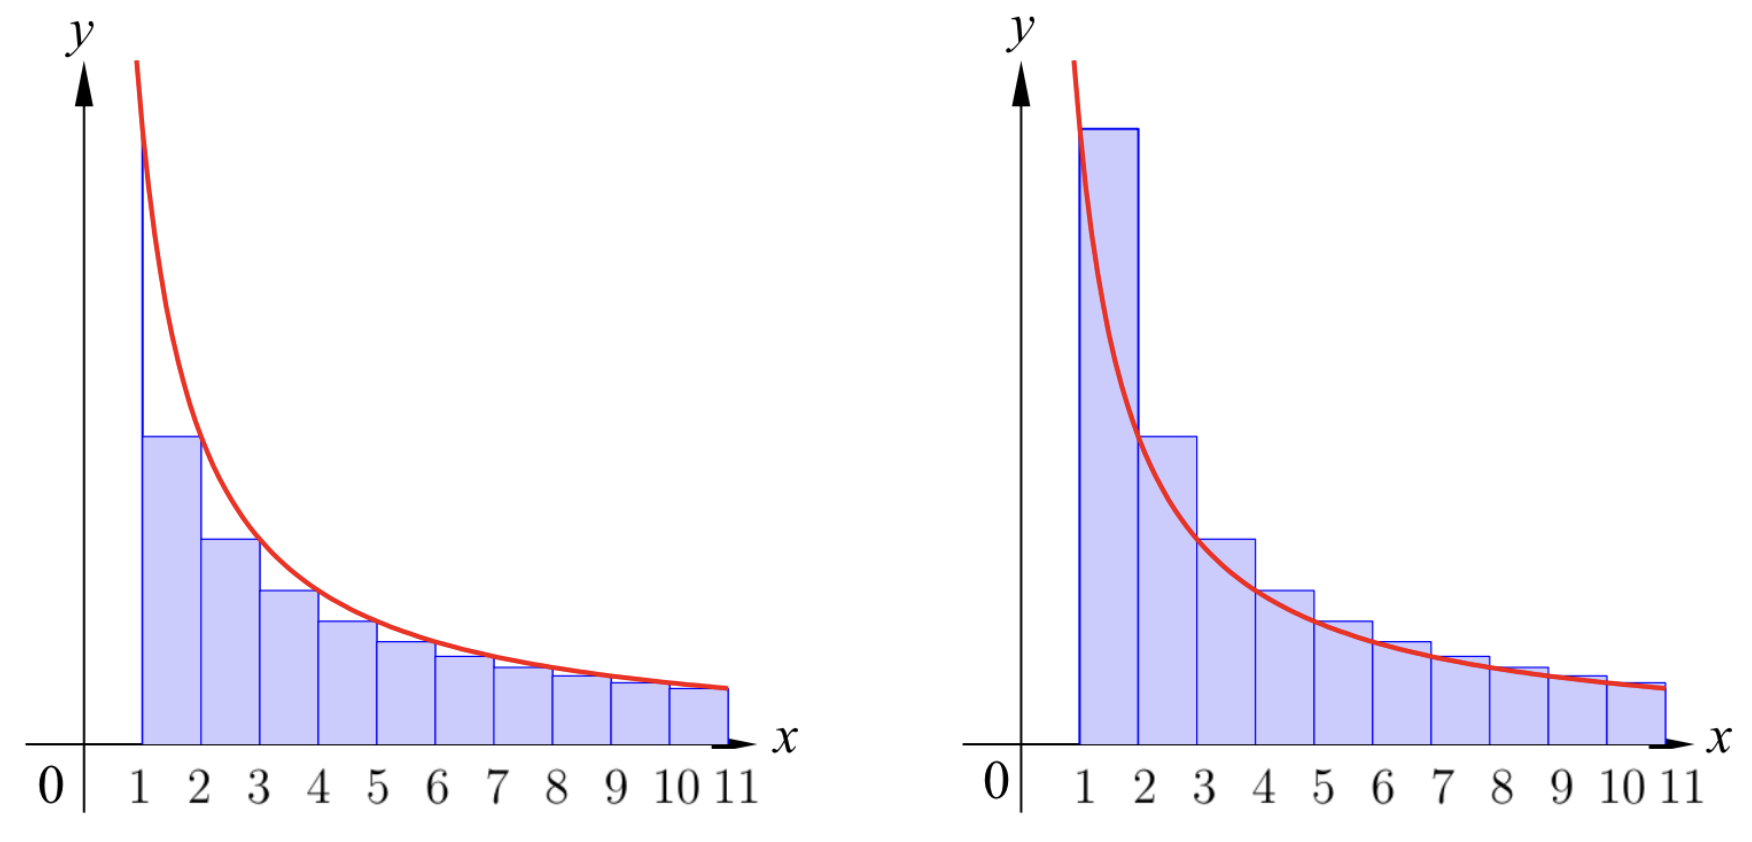
\includegraphics[scale=0.2]{Picture48.png}
\caption{The integral test.\fa}\label{figure48}
\end{figure}

Let us now use the integral test to determine the convergence of the $p$-series.
\begin{theorem}{p-Series}
Let $p$ be a positive number. The $p$-series $\di\sum_{n=1}^{\infty}\frac{1}{n^p}$ is convergent if and only if $p>1$.

\end{theorem}
\begin{myproof}{Proof}
Define the function $f:[1,\infty)\to\mathbb{R}$ by 
\[f(x)=\frac{1}{x^p}.\] Then $f$ is a continuous function that decreases monotonically to 0. By Example \ref{ex230227_10}, the improper integral $\di \int_1^{\infty}\frac{1}{x^p}dx$ is convergent if and only if $p>1$. By integral test, the series $\di\sum_{n=1}^{\infty}\frac{1}{n^p}$ is convergent if and only if $p>1$.
\end{myproof}

\begin{example}{}
The series $\di\sum_{n=1}^{\infty}\frac{1}{\sqrt{n}}$ is divergent since it is a $p$-series with $p=\frac{1}{2}\leq 1$.
\end{example}
\begin{remark}
{Integral Approximation to Partial Sums}
Given that $f:[1,\infty)\to\mathbb{R}$ is a continuous function that monotonically decreases to 0, let 
\[s_n=\sum_{k=1}^n f(k),\hspace{1cm} t_n=\int_1^nf(x)dx.\] 
From  the proof of the integral test, we have
\[t_n+f(n+1)\leq s_n\leq a_1+t_n.\]This implies that
\[f(n+1)\leq s_n-t_n\leq a_1,\]which gives bounds for the error when   the partial sum $s_n=\di\sum_{k=1}^na_k$ is approximated by the integral $\di\int_1^nf(x)dx$.
When the improper integral $\di\int_1^{\infty}f(x)dx$ is convergent, the sum $\di\sum_{n=1}^{\infty}a_n$ is also convergent. In this case, the sum of the infinite series satisfies
\[\int_1^{\infty}f(x)dx\leq \sum_{n=1}^{\infty}a_n\leq \int_1^{\infty}f(x)dx+a_1.\]
 If we use $s_n$ to approximate the sum $s=\di\sum_{n=1}^{\infty}a_n$, the error is
\[s-s_n=\sum_{k=n+1}^{\infty}a_k.\]
The same reasoning shows that if $n\geq 1$,
\[\int_{n+1}^{\infty}f(x)dx\leq s-s_n\leq\int_n^{\infty}f(x)dx.\]
\end{remark}

\begin{example}[label=ex230228_7]{Euler's Constant}
We can prove that the limit
\[\lim_{n\to\infty}\left(1+ \frac{1}{2}+\cdots+\frac{1}{n}-\ln n\right)\]exists as follows. Let
\[c_n=1+ \frac{1}{2}+\cdots+\frac{1}{n}-\ln n.\] Then
\[\ln n=\int_1^n\frac{1}{x}dx\leq \int_1^2\frac{1}{x}dx+\cdots+\int_{n-1}^{n}\frac{1}{x}dx
\leq 1+ \frac{1}{2}+\cdots+\frac{1}{n-1}.\]
Therefore, $c_n\geq 0$ for all $n\geq 1$. On the other hand,
\[c_{n+1}-c_n=\frac{1}{n+1}-\ln (n+1)+\ln n=\frac{1}{n+1}-\int_n^{n+1}\frac{1}{x}dx\leq 0.\]Hence, $\{c_n\}$ is a decreasing sequence that is bounded below by 0. By monotone convergence theorem, $\{c_n\}$ converges to a limit $\gamma$. This number \[\gamma=\lim_{n\to\infty}\left(1+ \frac{1}{2}+\cdots+\frac{1}{n}-\ln n\right)\] is called the Euler-Mascheroni constant, or simply as Euler's constant. It is an important constant in mathematics. Numerically, it is equal to
\[0.577215664901532\]correct to 15 decimal places.

\end{example}

Now we return to the comparison test. 
Using Theorem \ref{230227_3}, we obtain the following   test for nonnegative series.
\begin{theorem}{Comparison Test}
Let $\di\sum_{n=1}^{\infty}a_n$ and $\di\sum_{n=1}^{\infty}b_n$ be two series satisfying
\[0\leq a_n\leq b_n\hspace{1cm}\text{for all}\;n\geq 1.\]
\begin{enumerate}[1.]
\item
If $\di\sum_{n=1}^{\infty}b_n$ is convergent, $\di\sum_{n=1}^{\infty}a_n$ is convergent.
\item
If $\di\sum_{n=1}^{\infty}a_n$ is divergent, $\di\sum_{n=1}^{\infty}b_n$ is divergent.
\end{enumerate}
\end{theorem}
\begin{myproof}{Proof}
Let
$s_n=a_1+\ldots+a_n$ and $t_n=b_1+\ldots+b_n$  be respectively the $n^{\text{th}}$ partial sums of the series $\di\sum_{n=1}^{\infty}a_n$ and $\di\sum_{n=1}^{\infty}b_n$.   Then $\{s_n\}$ and $\{t_n\}$ are increasing sequences and \[s_n\leq t_n.\]
\begin{enumerate}[1.]\item 
If $\di\sum_{n=1}^{\infty}b_n$ is convergent, the sequence $\{t_n\}$ is bounded above. Then the sequence $\{s_n\}$  is also bounded above. Hence, $\di\sum_{n=1}^{\infty}a_n$ is convergent.
\item 
If $\di\sum_{n=1}^{\infty}a_n$ is divergent, the sequence $\{s_n\}$ is not bounded above. Then the sequence $\{t_n\}$  is also not bounded above. Hence, $\di\sum_{n=1}^{\infty}b_n$ is divergent.
\end{enumerate}
\end{myproof}

\begin{example}[label=ex230227_6]{}
Determine the convergence of the series 
\[\sum_{n=1}^{\infty}\frac{2^n}{3^n-1}.\]

\end{example}
\begin{solution}{Solution}
For $n\geq 1$, 
\[3^n-1\geq \frac{1}{2}\times 3^n.\]
Therefore,
\[\frac{2^n}{3^n-1}\leq   \frac{2^{n+1 }}{3^n}.\]Since the series \[\sum_{n=1}^{\infty}\frac{2^{n+1}}{3^n}=2\sum_{n=1}^{\infty}\frac{2^{n}}{3^n}\] is a geometric series with $r=2/3$, it is convergent. By comparison test, the series $\di\sum_{n=1}^{\infty}\frac{2^n}{3^n-1}$ is convergent.
\end{solution}

\begin{example}[label=ex230227_7]{}
Determine the convergence of the series 
\[\sum_{n=1}^{\infty}\frac{n}{n\sqrt{n}+1}.\]

\end{example}
\begin{solution}{Solution}For $n\geq 1$,\[
\frac{n}{n\sqrt{n}+1}\geq\frac{n}{n\sqrt{n}+n\sqrt{n}}=\frac{1}{2 \sqrt{n}}.\]
Since the series $\di\sum_{n=1}^{\infty}\frac{1}{\sqrt{n}}$ is a $p$-series with $p=1/2\leq 1$, it is divergent. So   the series $\di\sum_{n=1}^{\infty}\frac{1}{2\sqrt{n}}$ is also divergent. By comparison test, the series
$\di \sum_{n=1}^{\infty}\frac{n}{n\sqrt{n}+1}$ is divergent.
\end{solution}

In applying the comparison test, we need to identify the correct series to compare to, and prove some strict inequalities. In Example \ref{ex230227_6}, we compare  $a_n=\di \frac{2^n}{3^n-1}$ to $b_n=\di \frac{2^n}{3^n}$, since $2^n$ and $3^n$ are the leading terms of the numerator and the denominator of $a_n$ when $n$ is large. Since we know that the series $\di\sum_{n=1}^{\infty}\frac{2^n}{3^n}$ is convergent, we need to prove that $a_n $ is up to a constant, less than or equal to $b_n$, in order to use the comparison test to conclude that $\di\sum_{n=1}^{\infty}a_n$ is convergent.

Simiarly, for Example \ref{ex230227_7}, we compare  $a_n=\di\frac{n}{n\sqrt{n}+1}$ to $\di b_n=\frac{n}{n\sqrt{n}}$ since $n$ and $n\sqrt{n}$ are respectively the leading terms of the numerator and denominator of $a_n$. Since $\di\sum_{n=1}^{\infty}b_n$ is divergent, so we want to conclude that $\di\sum_{n=1}^{\infty}a_n$ is divergent. For this, we need to show that $a_n$ is larger than a constant times $b_n$.

Proving strict inequalities is tedious, and we see that it might not be necessary. In fact, we obtain the series to compare to by investigating the leading terms. This is somehow a limit. Hence, we can replace the comparison test by limit comparison test.  


\begin{theorem}{Limit Comparison Test}
Given the two series  $\di\sum_{n=1}^{\infty}a_n$ and $\di\sum_{n=1}^{\infty}b_n$ that satisfy the following conditions.
 
\begin{enumerate}[(i)]
\item $a_n\geq 0$ and $b_n>0$ for all $n\in\mathbb{Z}^+$.
\item The limit $\di L=\lim_{n\to\infty} \frac{a_n}{b_n} $ exists and is finite. 
\end{enumerate}Since $\di \frac{a_n}{b_n}\geq 0$, we must have $L\geq 0$.
\begin{enumerate}[1.]
\item If $L=0$, and the  series $\di\sum_{n=1}^{\infty}b_n$ is convergent, then the series $\di\sum_{n=1}^{\infty}a_n$ is convergent.
\item If  $L>0$,   the  series $\di\sum_{n=1}^{\infty}a_n$ is convergent if and only if the series $\di\sum_{n=1}^{\infty}b_n$ is convergent.
\end{enumerate}

\end{theorem} The   condition  (ii)  says that when $n$ is large, $a_n$ is smaller than or equal to a multiple of   $b_n$.  
\begin{myproof}{Proof}
First consider the case where $L=0$.
By definition of limit with $\varepsilon=1$, there is a positive integer $N$ such that for all $n\geq N$, 
\[\left| \frac{a_n}{b_n} \right|< 1.\]
Therefore,
\[0\leq a_n\leq b_n\hspace{1cm}\text{for all}\; n\geq N.\]
Since the series $\di\sum_{n=1}^{\infty}b_n$ is convergent,  the series $\di\sum_{n=N}^{\infty}  b_n$ is convergent. Then comparison test implies that the series $\di \sum_{n=N}^{\infty} a_n $ is convergent. Therefore, the series $\di \sum_{n=1}^{\infty} a_n $ is convergent.  

Now for the case $L>0$, take $\varepsilon=L/2$. There is a positive integer $N$ such that for all $n\geq N$, 
\[\left| \frac{a_n}{b_n} -L\right|<\frac{L}{2}.\]
This implies that
\[0\leq \frac{L}{2}b_n \leq a_n\leq\frac{3L}{2} b_n\hspace{1cm}\text{for all}\; n\geq N.\]
Comparison test then shows that  the  series $\di\sum_{n=1}^{\infty}a_n$ is convergent if and only if the series $\di\sum_{n=1}^{\infty}b_n$ is convergent.
\end{myproof}

\begin{example}{\linkt Example \ref{ex230227_6} Revisited}
For the series $\di \sum_{n=1}^{\infty}\frac{2^n}{3^n-1}$ considered in Example \ref{ex230227_6}, we take $a_n=\di\frac{2^n}{3^n-1}$ and $\di b_n=\frac{2^n}{3^n }$.\be Then
\[\lim_{n\to\infty}\frac{a_n}{b_n}=\lim_{n\to\infty} \frac{1}{1-\di\frac{1}{3^n}}=1.\] 
 Since the series $\di\sum_{n=1}^{\infty}\frac{2^n}{3^n}$  is convergent, the series $\di\sum_{n=1}^{\infty}\frac{2^n}{3^n-1}$ is convergent.
\end{example2}

\begin{example}{\linkt Example \ref{ex230227_7} Revisited}
For the series $\di \sum_{n=1}^{\infty}\frac{n}{n\sqrt{n}+1}$ considered in Example \ref{ex230227_7}, we take $a_n=\di\frac{n}{n\sqrt{n}+1}$ and $\di b_n=\frac{1}{\sqrt{n}}$.  Then
\[\lim_{n\to\infty}\frac{a_n}{b_n}=\lim_{n\to\infty} \frac{1}{1+\di \frac{1}{n\sqrt{n}}}=1.\] 
 Since the series $\di\sum_{n=1}^{\infty}\frac{1}{\sqrt{n}}$  is divergent, the series $\di\sum_{n=1}^{\infty}\frac{n}{n\sqrt{n}+1}$ is divergent.
\end{example}


Let us now turn to series that can have negative terms. First we formulate a Cauchy criterion for convergence of series. Recall that a sequence $\{s_n\}$ is a Cauchy sequence if for every $\varepsilon>0$, there is a positive integer $N$ so that for all $m\geq n\geq N$, 
\[|s_m-s_n|<\varepsilon.\]
Applying the Cauchy criterion for convergence of sequences (see Theorem \ref{23020602}), and the fact that if $m\geq  n>1$,
\[s_m-s_{n-1}=a_{n}+a_{n+1}+\cdots+a_m,\] we obtain the following Cauchy criterion for convergence of infinite series.
\begin{theorem}{Cauchy Criterion for Infinite Series}
An infinite series $\di\sum_{n=1}^{\infty}a_n$ is convergent if and only if for every $\varepsilon>0$, there is a positive integer $N$ such that for all $m\geq n\geq N$,
\[|a_n+a_{n+1}+\cdots+a_m|<\varepsilon.\]
\end{theorem}

Using this, we can prove the following.


\begin{theorem}[label=230227_11]{}
If the series $\di\sum_{n=1}^{\infty}|a_n|$ is convergent, then the series $\di\sum_{n=1}^{\infty}a_n$ is convergent.
\end{theorem}
\begin{myproof}{Proof}
Given $\varepsilon>0$, since the series $\di\sum_{n=1}^{\infty}|a_n|$ is convergent, there is a positive integer $N$ such that for all $m\geq n\geq N$,
\[|a_n|+|a_{n+1}|+\cdots+|a_m|=\left||a_n|+|a_{n+1}|+\cdots+|a_m|\right|<\varepsilon.\] 
By triangle inequaltiy, we find that for $m\geq n\geq N$, 
\[|a_n+a_{n+1}+\cdots+a_m|<|a_n|+|a_{n+1}|+\cdots+|a_m|<\varepsilon.\]
Using Cauchy criterion, we conclude that the series $\di\sum_{n=1}^{\infty}a_n$ is convergent.
\end{myproof}

The converse of Theorem \ref{230227_11} is not true. Namely, there exists series $\di\sum_{n=1}^{\infty}a_n$ which is  convergent but the corresponding absolute series $\di\sum_{n=1}^{\infty}|a_n|$ is not convergent. Therefore, let us make the following definitions.
\begin{definition}{Absolute Convergence and Conditional Convergence}
Given that the series $\di\sum_{n=1}^{\infty}a_n$ is convergent.
\begin{enumerate}[1.]
\item
We say that the series $\di\sum_{n=1}^{\infty}a_n$ {\bf converges absolutely} if the series $\di\sum_{n=1}^{\infty}|a_n|$ is convergent.
\item We say that the series $\di\sum_{n=1}^{\infty}a_n$ {\bf converges conditionally} if the series $\di\sum_{n=1}^{\infty}|a_n|$ is divergent.
\end{enumerate}
\end{definition}

 

\begin{example}{}
If $p>1$, the series $\di\sum_{n=1}^{\infty}\frac{(-1)^n}{n^p}$ converges absolutely.
\end{example}

From the limit comparison test, we have the following. 
\begin{theorem}{Limit Comparison Test II}
Given the  series  $\di\sum_{n=1}^{\infty}a_n$, assume that there is a series $\di\sum_{n=1}^{\infty}b_n$ such that $b_n>0$ for all $n\in\mathbb{Z}^+$, and the limit $\di L=\lim_{n\to\infty} \frac{|a_n|}{b_n} $ exists and is finite. 
 If  the series $\di\sum_{n=1}^{\infty}b_n$ is convergent, then the  series $\di\sum_{n=1}^{\infty}a_n$ converges absolutely.
 
\end{theorem}

\begin{example}{}
Show that the series
\[\sum_{n=1}^{\infty} \frac{2^n+(-1)^n3^n}{5^n+1}\] is convergent.
\end{example}
\begin{solution}{Solution}
Let
\[a_n=\frac{2^n+(-1)^n3^n}{5^n+1},\hspace{1cm}b_n=\frac{3^n}{5^n}.\]
Then $b_n>0$ for all $n\in\mathbb{Z}^+$ and $\di\sum_{n=1}^{\infty}b_n$ is convergent. Now,
\[\lim_{n\to\infty}\frac{|a_n|}{b_n}=\lim_{n\to\infty}\frac{\di 1+(-1)^n\left(\frac{2}{3}\right)^n}{1+\di \frac{1}{5^n}}=1.\]
Therefore, the series $\di \sum_{n=1}^{\infty} \frac{2^n+(-1)^n3^n}{5^n+1}$ converges absolutely, and thus is convergent.
\end{solution}

 To give  an example of series that converges conditionally, let us   discuss a convergence test for a special class of series called alternating series.

\begin{definition}{Alternating Series}
A series of the form \[\sum_{n=1}^{\infty}(-1)^{n-1}b_n=b_1-b_2+b_3-b_4+\cdots+b_{2n-1}-b_{2n}+\cdots,\]where $b_n\geq 0$ for all $n\geq 1$, is called an alternating series.
\end{definition}

\begin{example}[label=ex230227_12]{}
The series 
\[1-\frac{1}{2}+\frac{1}{3}-\frac{1}{4}+\cdots\] is an alternating series.
\end{example} 
A necessary condition for an alternating series $\di\sum_{n=1}^{\infty}(-1)^{n-1}b_n$ to be convergent is $\di\lim_{n\to\infty}b_n=0$. The following theorem says that if $\{b_n\}$ is also decreasing, then the alternating series is convergent. 

\begin{theorem}[label=230227_15]{Alternating Series Test}
If  $\{b_n\}$ is a monotonically decreasing sequence with $\di\lim_{n\to \infty}b_n=0$, the alternating series $\di\sum_{n=1}^{\infty}(-1)^{n-1}b_n$ is convergent.
\end{theorem}
\begin{myproof}{Proof}Since $\{b_n\}$ decreases monotonically to 0, $b_n\geq 0$ for all $n\in\mathbb{Z}^+$. 
Let $a_n=(-1)^{n-1}b_n$ be the $n^{\text{th}}$ term of the series $\di\sum_{n=1}^{\infty}(-1)^{n-1}b_n$ , and let $s_n=a_1+a_2+\cdots+a_n$ be the $n^{\text{th}}$ partial sum. We are given that 
\[b_1\geq b_2\geq \cdots\geq b_n\geq b_{n+1}\cdots.\]
Therefore,
\begin{align*}
s_{2n+1}&= s_{2n-1}+a_{2n}+a_{2n+1}=s_{2n-1}-(b_{2n}-b_{2n+1})\leq s_{2n-1},\\
s_{2n+2}&=s_{2n}+a_{2n+1}+a_{2n+2} =s_{2n}+(b_{2n+1}-b_{2n+2})\geq s_{2n}. 
\end{align*}This shows that $\{s_{2n-1}\}$ is a decreasing sequence and $\{s_{2n }\}$ is an increasing sequence.
Since 
\[s_{2n }=s_{2n-1}-b_{2n},\]
we find that 
\[s_2\leq s_{2n}\leq s_{2n-1}\leq s_1.\]
Namely, the sequence $\{s_{2n-1}\}$ is bounded below by $s_2$, while the sequence $\{s_{2n}\}$ is bounded above by $s_1$. By the monotone convergence theorem, the limits
\[s_o=\lim_{n\to\infty}s_{2n-1}\hspace{1cm}\text{and}\hspace{1cm}s_e=\lim_{n\to\infty}s_{2n}\] exist.  Since
\[-b_{2n}=a_{2n}=s_{2n}-s_{2n-1},\] 
taking the $n\to \infty$ limits give
\[s_o=s_e.\]\bp
This proves that the sequence $\{s_n\}$ has a limit $s=s_0=s_e$, and thus the alternating series $\di\sum_{n=1}^{\infty}(-1)^{n-1}b_n$ is convergent.


\end{myproof}
Notice that the sum of the alternating series $s=\di\sum_{n=1}^{\infty}(-1)^{n-1}b_n$ is the least upper bound of $\{s_{2n}\}$, and the greatest lower bound of $\{s_{2n-1}\}$.  




\begin{remark}{Approximating   the Sum of An Alternating Series}
If $\{b_n\}$ is a sequence that decreases monotonically to 0, the alternating series $\di\sum_{n=1}^{\infty}(-1)^{n-1}b_n$ converges to a sum $s$. If 
\[s_n=\sum_{k=1}^n(-1)^{k-1}b_k\] is the $n^{\text{th}}$ partial sum, then the error in approximating $s$ by $s_n$ is
\[s-s_n=\sum_{k=n+1}^{\infty}(-1)^{k-1}b_k,\] which is also an alternating series. From the proof of Theorem \ref{230227_15}, we obtain a simple estimate
\[|s-s_n|\leq |b_{n+1}|.\]
\end{remark}

\begin{example}[label=ex230227_13]{}
For the alternating   series 
\[\sum_{n=1}^{\infty}\frac{(-1)^{n-1}}{n}=1-\frac{1}{2}+\frac{1}{3}-\frac{1}{4}+\cdots\] in Example \ref{ex230227_12}, $b_n=\di\frac{1}{n}$.  Since $\{b_n\}$ decreases monotonically to 0, by the alternating series test, the series \be \[ \sum_{n=1}^{\infty}\frac{(-1)^{n-1}}{n}=1-\frac{1}{2}+\frac{1}{3}-\frac{1}{4}+\cdots\]  is convergent.   
  Since the harmonic series $\di\sum_{n=1}^{\infty}\frac{1}{n}$ is divergent, the series $\di \sum_{n=1}^{\infty}\frac{(-1)^{n-1}}{n}$ converges conditionally.
\end{example2}

 
\begin{example}[label=ex230227_14]{}
For any $0<p\leq 1$, the sequence $\{1/n^p\}$ decreases to 0 montonically. Hence, the alternating series $\di \sum_{n=1}^{\infty}\frac{(-1)^{n-1}}{n^p}$ is convergent. Since the series $\di\sum_{n=1}^{\infty}\frac{1}{n^p}$ is divergent,  the series   $\di \sum_{n=1}^{\infty}\frac{(-1)^{n-1}}{n^p}$ converges conditionally.
\end{example} 



Now we turn to two useful tests that are used for testing convergence of power series. They both based on comparisons with geometric series. We first prove the following.

\begin{theorem}[label=230227_22]{}
Let $\{a_n\}$ be a sequence of positive numbers. Then
\[\liminf_{n\to\infty}\frac{a_{n+1}}{a_n}\leq\liminf_{n\to\infty}\sqrt[n]{a_n}\leq \limsup_{n\to\infty}\sqrt[n]{a_n}\leq \limsup_{n\to\infty}\frac{a_{n+1}}{a_n}.\]
Hence, if the limit $\di\lim_{n\to\infty}\frac{a_{n+1}}{a_n}$ exists, the limit $\di\lim_{n\to\infty}\sqrt[n]{a_n}$ also exists, and the two limits are equal.
\end{theorem}Since $a_n>0$ for all $n\in\mathbb{Z}^+$, all the four limits in the theorem are nonnegative. \begin{myproof}{Proof}

If $\{c_n\}$ is a sequence of postive numbers,  it is easy to verify that
\[\sup \left\{\frac{1}{c_n}\right\}=\frac{1}{\inf\{c_n\}},\hspace{1cm}\inf \left\{\frac{1}{c_n}\right\}=\frac{1}{\sup\{c_n\}}.\] \bp Therefore, if we prove that
\begin{equation}\label{eq230227_20}\limsup_{n\to\infty}\sqrt[n]{a_n}\leq \limsup_{n\to\infty}\frac{a_{n+1}}{a_n},\end{equation} 
then 
\[\liminf_{n\to\infty}\frac{a_{n+1}}{a_n}\leq\liminf_{n\to\infty}\sqrt[n]{a_n}\] follows by applying \eqref{eq230227_20} to the reciprocal sequence $\{1/a_n\}$. 
From Proposition \ref{230227_11}, we have the inequality $\di \liminf_{n\to\infty}\sqrt[n]{a_n}\leq \limsup_{n\to\infty}\sqrt[n]{a_n}$. 
Hence, we only need to prove  \eqref{eq230227_20}.

 If $\di  \limsup_{n\to\infty}\frac{a_{n+1}}{a_n}=\infty$, there is nothing to prove. Hence, we consider the case
\[u= \limsup_{n\to\infty}\frac{a_{n+1}}{a_n}\] is finite. Given $\varepsilon>0$, there is a positive integer $N$ such that
\[\frac{a_{n+1}}{a_n}<u+ \varepsilon \hspace{1cm}\text{for all}\;n\geq N.\]
By induction, we find that
\[a_n\leq a_N\left(u+ \varepsilon\right)^{n-N}\hspace{1cm}\text{for all}\;n\geq N.\]Let 
$c=a_N(u+\varepsilon)^{-N}$. 
Then 
\[\sqrt[n]{a_n}\leq c^{1/n}(u+\varepsilon)\hspace{1cm}\text{for all}\;n\geq N.\]
This implies that
\[\limsup_{n\to\infty}\sqrt[n]{a_n}\leq \limsup_{n\to\infty}c^{1/n}(u+\varepsilon)=(u+\varepsilon)\lim_{n\to\infty}c^{1/n}=(u+\varepsilon).\]
Since $\varepsilon>0$ is arbitrary, we conclude that
\[\limsup_{n\to\infty}\sqrt[n]{a_n}\leq u= \limsup_{n\to\infty}\frac{a_{n+1}}{a_n}.\]This completes the proof of the theorem.
\end{myproof}

Now we come to the proof of the root test.
\begin{theorem}[label=230227_23]{Root Test}
Given a series $\di\sum_{n=1}^{\infty}a_n$, let
\[\rho=\limsup_{n\to\infty}\sqrt[n]{|a_n|}.\]
\begin{enumerate}[1.]
\item
If $\rho<1$, the series $\di\sum_{n=1}^{\infty}a_n$ converges absolutely.
\item If $\rho>1$,  the series $\di\sum_{n=1}^{\infty}a_n$ is divergent.
\item If $\rho=1$, the test is inconclusive.
\end{enumerate}
\end{theorem}\begin{myproof}{Proof}
If $\rho<1$, take $\di\varepsilon=\frac{1-\rho}{2}$ in (b)(i) of Theorem \ref{230226_5}. There is a positive integer $N$ such that 
\[\sqrt[n]{|a_n|}<\rho+\varepsilon=\rho_1\hspace{1cm}\text{for all}\;n\geq N.\]
Thus, we have
\[|a_n|<\rho_1^n\hspace{1cm}\text{for all}\;n\geq N.\]Notice that
\[\rho_1=\frac{1+\rho}{2}<1.\]Therefore, the geometric series $\di\sum_{n=N}\rho_1^n$ is convergent. By comparison test, the series $\di\sum_{n=1}^{\infty}|a_n|$ is convergent. Thus, the series $\di\sum_{n=1}^{\infty}a_n$ converges absolutely.

If $\rho>1$,  take $\di\varepsilon=\frac{ \rho-1}{2}$ in (b)(ii) of Theorem \ref{230226_5}. There are positive  integers $n_1, n_2, \ldots$ such that $1\leq n_1<n_2<\ldots$ and
\[\sqrt[\leftroot{-3}\uproot{ 5} n_k]{|a_{n_k}|}>\rho-\varepsilon=\rho_2\hspace{1cm}\text{for all}\; k\in\mathbb{Z}^+.\]\bp
Thus, we have
\begin{equation}\label{eq230228_1}|a_{n_k}|>\rho_2^{n_k}\hspace{1cm}\text{for all}\;k\in\mathbb{Z}^+.\end{equation}
Since
\[\rho_2=\frac{1+\rho}{2}>1,\]and $n_k\to\infty$ as $k\to\infty$, we find that 
$\di\lim_{k\to\infty}\rho_2^{n_k}=\infty$. In other words, the sequence $\{\rho_2^{n_k}\}$ is not bounded above. Eq. \eqref{eq230228_1} then implies that $\{|a_{n_k}|\}$ is also not bounded above. Therefore, the limit $\di\lim_{n\to\infty}a_n$ is not zero. Hence, the series $\di\sum_{n=1}^{\infty}a_n$ is divergent.

Now, let us look at some examples where $\rho=1$. First, notice that
\begin{equation}\label{eq230305_7}\lim_{n\to\infty}\sqrt[n]{n}=\lim_{n\to\infty}\exp\left(\frac{\ln n}{n}\right)=\exp\left(\lim_{x\to\infty}\frac{\ln x}{x}\right)=e^0=1.\end{equation}
For the $p$-series $\di\sum_{n=1}^{\infty}\frac{1}{n^p}$, $a_n=n^{-p}$. Thus,
\[\rho=\lim_{n\to\infty}\sqrt[n]{n^{-p}}=\left(\lim_{n\to\infty}\sqrt[n]{n}\right)^{-p}=1.\]
But we have seen that the $p$-series is divergent if $p\leq 1$, and it is convergent when $p>1$. This shows that the root test is conclusive when $\rho=1$.
\end{myproof} 

\begin{example}{}
Determine the convergence of the  series 
$\di\sum_{n=1}^{\infty}\left(\frac{1-n}{2n+1}\right)^n$.
 
\end{example}
\begin{solution}{Solution}
Applying root test, 
\[\rho=\limsup_{n\to\infty}\sqrt[\leftroot{-5}\uproot{15} n]{\left|\left(\frac{1-n}{2n+1}\right)^n\right|}=\lim_{n\to\infty}\frac{n-1}{2n+1}=\frac{1}{2}.\]
Since $\rho<1$, we find that the series   is convergent.
\end{solution}

Finally, we have the ratio test.
\begin{theorem}[label=230305_4]{Ratio Test}
Given a series $\di\sum_{n=1}^{\infty}a_n$ with $a_n\neq 0$ for all $n\in\mathbb{Z}^+$, let
\[r=\liminf_{n\to\infty}\left|\frac{a_{n+1}}{a_n}\right|,\hspace{1cm}R=\limsup_{n\to\infty}\left|\frac{a_{n+1}}{a_n}\right|.\]
\begin{enumerate}[1.]
\item
If $R<1$, the series $\di\sum_{n=1}^{\infty}a_n$ converges absolutely.
\item If $r>1$,  the series $\di\sum_{n=1}^{\infty}a_n$ is divergent.
\item If $r\leq 1\leq R$, the test is inconclusive.
\end{enumerate}
\end{theorem}\begin{myproof}{Proof}
 
If $R<1$, Theorem \ref{230227_22} implies that $\rho=\di\limsup_{n\to\infty}\sqrt[n]{|a_n|}<1$. Theorem \ref{230227_23} implies that $\di\sum_{n=1}^{\infty}a_n$ converges absolutely.
 
If $r>1$, Theorem \ref{230227_22} implies that $\rho=\di\limsup_{n\to\infty}\sqrt[n]{|a_n|}>1$. Theorem \ref{230227_23} implies that $\di\sum_{n=1}^{\infty}a_n$  is divergent.
 
The $p$-series $\di\sum_{n=1}^{\infty}\frac{1}{n^p}$ provides examples of $r=R=1$, but the series is convergent if $p>1$, divergent when $p\leq1 $. Hence, ratio test is also inconclusive when $r\leq 1\leq R$.

 \end{myproof}
Ratio test is useful to determine the convergence of power series. We are going to study this in Chapter 6.

\begin{example}
{}
Determine whether the series is convergent.
\begin{enumerate}[(a)]
\item $\di \sum_{n=1}^{\infty}(-1)^{n-1}\frac{2^n}{n+1}$
\item  $\di \sum_{n=1}^{\infty}(-1)^{n-1}\frac{n+1}{2^n}$

\end{enumerate}
\end{example}
\begin{solution}{Solution}
\begin{enumerate}[(a)]
\item Using  ratio test with $\di a_n=(-1)^{n-1}\frac{2^n}{n+1}$, we find that
\[r=R=\lim_{n\to\infty}\left|\frac{a_{n+1}}{a_n}\right|=\lim_{n\to\infty}\frac{2^{n+1}}{n+2}\times\frac{n+1}{2^n}=2\lim_{n\to\infty}\frac{n+1}{n+2}=2.\]
Therefore, the series $\di \sum_{n=1}^{\infty}(-1)^{n-1}\frac{2^n}{n+1}$ is divergent.
\item Using  ratio test with $\di a_n=(-1)^{n-1}\frac{n+1}{2^n}$, we find that
\[r=R=\lim_{n\to\infty}\left|\frac{a_{n+1}}{a_n}\right|=\lim_{n\to\infty}\frac{n+2}{2^{n+1}}\times\frac{2^n}{n+1}=\frac{1}{2}\lim_{n\to\infty}\frac{n+2}{n+1}=\frac{1}{2}.\]
Therefore, the series $\di \sum_{n=1}^{\infty}(-1)^{n-1}\frac{n+1}{2^n}$ is convergent.

\end{enumerate}
\end{solution}

\begin{highlight}{Convergence Tests}
In this section, we have explored various strategies to determine the convergence of a series $\di\sum_{n=1}^{\infty}a_n$. We make a summary as follows. This is a useful manual for beginners, but it is not binding.

\begin{enumerate}[1.]
\item   Check whether $\di\lim_{n\to\infty}a_n$ is 0. If not, the series $\di\sum_{n=1}^{\infty}a_n$ is divergent.\end{enumerate}\end{highlight}\begin{highlight}{}\begin{enumerate}[1.] 
\item[2.] Check whether it is a geometric series $\di\sum_{n=1}^{\infty}ar^{n-1}$ or a $p$-series $\di\sum_{n=1}^{\infty}\frac{1}{n^p}$. A geometric series $\di\sum_{n=1}^{\infty}ar^{n-1}$ is convergent if and only if $|r|<1$. A $p$-series $\di\sum_{n=1}^{\infty}\frac{1}{n^p}$ is convergent if and only if $p>1$.
\item[3.] If $a_n$ contains powers of $n$ and functions such as $\ln n$, use integral test.
\item[4.] If  $a_n$ involves only expressions of the form $r^n$ for more than one $r$, do limit comparison test to compare with a geometric series.
\item[5.] If  $a_n$ is a rational function of powers of  $n$, do limit comparison test with a $p$-series.
\item[6.]  For alternating series which does not converge absolutely, check whether alternating series test can be applied.
\item[7.] If $a_n=b_n^n$ for each $n\in\mathbb{Z}^+$, and $\di\limsup_{n\to\infty}b_n$ exists, use root test.
\item[8.]  If $a_n$ is a product of a rational function of powers of $n$ and expressions of the form $r^n$, use ratio test.
\end{enumerate}
\end{highlight}

Finally, we want to prove the following useful fact.
\begin{theorem}[label=230306_1]{}
Let $r$ be a real number with $|r|<1$. For any real number $\alpha$, \[\lim_{n\to\infty}n^{\alpha}r^n=0.\]
\end{theorem}\begin{myproof}{Proof}
If $r=0$, the limit is trivial. Hence, we consider the case $|r|<1$ and $r\neq 0$.

If $\alpha\leq 0$, the statement is also easy to prove since $\di\lim_{n\to\infty}r^n=0$ and \bp\[\di\lim_{n\to\infty}n^{\alpha}=\begin{cases}0,\quad&\text{if}\;\alpha<0, \\1, \quad & \text{if}\;\alpha=0.\end{cases}\]


The highly nontrivial case is when $\alpha>0$. In this case, $\di\lim_{n\to\infty}n^{\alpha}=\infty$. Since
\[n^{\alpha}|r|^n=n^{\alpha}e^{n\ln |r|},\]
and $\ln |r|<0$, we can deduce that $\di \lim_{n\to\infty}n^{\alpha}|r|^n=0$ from $\di\lim_{x\to\infty}\frac{x^{\alpha}}{e^x}=0$. Nevertheless, let us present an alternative argument here which is interesting by its own. 

Consider the series $\di\sum_{n=1}^{\infty}n^{\alpha}r^n$ with $a_n=n^{\alpha}r^n$. When $|r|<1$ and $r\neq 0$,
\[\lim_{n\to\infty}\left|\frac{a_{n+1}}{a_n}\right|=\lim_{n\to\infty}|r|\left(\frac{n+1}{n}\right)^{\alpha}=|r|\left(\lim_{n\to\infty}\frac{n+1}{n}\right)^{\alpha}=|r|<1.\]
By ratio test, the  series $\di\sum_{n=1}^{\infty}n^{\alpha}r^n$ is convergent. Therefore,
\[\lim_{n\to\infty}n^{\alpha}r^n=\lim_{n\to\infty}a_n=0.\]
\end{myproof}
\vp
\noindent
{\bf \large Exercises  \thesection}
\setcounter{myquestion}{1}

\begin{question}{\themyquestion}
Determine whether the series $\di\sum_{n=1}^{\infty}\frac{n^2+1}{3n^2+n+1}$ is convergent.
\end{question}
\atc

\begin{question}{\themyquestion}
Let $p$ be a positive number. Show that the series $\di \sum_{n=1}^{\infty}\frac{\ln n}{n^p}$ is convergent if and only if $p>1$.
\end{question}
\atc

\begin{question}{\themyquestion}
Let $p$ be a positive number. Show that the series \[\sum_{n=1}^{\infty}(-1)^{n-1}\frac{\ln n}{n^p}\] is convergent.
\end{question}
\atc

\begin{question}{\themyquestion}
Determine whether the series is convergent.
\begin{enumerate}[(a)]
\item $\di \sum_{n=1}^{\infty}\frac{3^n+(-1)^n4^n}{5^n+2^n}$
\item  $\di \sum_{n=1}^{\infty}\frac{2^n-5^n}{4^n+3^n+1}$
\end{enumerate}
\end{question}
\atc


\begin{question}{\themyquestion}
Determine whether the series $\di\sum_{n=1}^{\infty}(-1)^{n-1}\frac{\sqrt{n}}{n+1}$ is convergent.
\end{question}
\atc
\begin{question}{\themyquestion}
Determine whether the series is convergent.
\begin{enumerate}[(a)]
\item $\di \sum_{n=1}^{\infty}\frac{2n\sqrt{n}+3}{5n^2-2}$
\item  $\di \sum_{n=1}^{\infty}\frac{4n^2-7}{6n^3\sqrt{n}+1}$
\end{enumerate}
\end{question}
\atc
\begin{question}{\themyquestion}
Use Theorem \ref{230227_22} to determine
\[\lim_{n\to\infty}\sqrt[n]{n!}.\]
\end{question}
\atc





\begin{question}{\themyquestion}
Determine whether the series is convergent.
\begin{enumerate}[(a)]
\item $\di \sum_{n=1}^{\infty}\left(\frac{2 \sqrt{n}-1}{\sqrt{n}+1}\right)^n$
\item  $\di \sum_{n=1}^{\infty}\left(\frac{2 \sqrt{n}-1}{3\sqrt{n}+1}\right)^n$
\end{enumerate}
\end{question}
\atc

\begin{question}{\themyquestion}
Determine whether the series is convergent.
\begin{enumerate}[(a)]
\item $\di \sum_{n=1}^{\infty}(-1)^{n-1}\frac{\sqrt{n}2^n}{3^n}$
\item  $\di \sum_{n=1}^{\infty}(-1)^{n-1}\frac{4^n}{3^nn^2}$
\end{enumerate}
\end{question}
 

\vp


\section{Rearrangement of Series}\label{sec5.3}
In this section, we want to explore more about the difference between a series that converges absolutely and one that converges conditionally.
 

Given a series $\di\sum_{n=1}^{\infty}a_n$ with terms $\{a_n\}$, define 
\begin{align*}
p_n&=\frac{|a_n|+a_n}{2}=\begin{cases}a_n,\hspace{0.7cm} &\text{if}\;a_n\geq 0,\\0,\quad &\text{if}\;a_n<0;\end{cases}\\q_n&=\frac{|a_n|-a_n}{2}=\begin{cases}-a_n,\quad &\text{if}\;a_n\leq 0,\\0,\quad &\text{if}\;a_n>0.\end{cases}.\end{align*}
Then $0\leq p_n\leq |a_n|$, $0\leq q_n\leq |a_n|$, and
\[|a_n|=p_n+q_n,\hspace{1cm}a_n=p_n-q_n.\]

\begin{example}[label=230228_4]{}
For the series $\di\sum_{n=1}^{\infty}\frac{(-1)^{n-1}}{n}=1-\frac{1}{2}+\frac{1}{3}-\frac{1}{4}+\cdots$,
\[p_{2n-1}=\frac{1}{2n-1},\quad p_{2n}=0;\hspace{1cm}q_{2n-1}=0,\hspace{1cm}q_{2n}=\frac{1}{2n}.\]
\end{example}

\begin{theorem}[label=230228_10]{}Let $\di\sum_{n=1}^{\infty}a_n$ be a convergent series.
\begin{enumerate}[1.]
\item 
If the series $\di\sum_{n=1}^{\infty}a_n$ converges absolutely, then the series $\di\sum_{n=1}^{\infty}p_n$ and the series $\di\sum_{n=1}^{\infty}q_n$ are convergent.
\item 
If the series $\di\sum_{n=1}^{\infty}a_n$ converges conditionally, then the series $\di\sum_{n=1}^{\infty}p_n$ and the series $\di\sum_{n=1}^{\infty}q_n$ are divergent.
 
\end{enumerate}
\end{theorem}
\begin{myproof}{Proof}
First we show that  the two series $\di\sum_{n=1}^{\infty}p_n$ and $\di\sum_{n=1}^{\infty}q_n$ can only be both convergent or both divergent.
We have
\[p_n=a_n+q_n,\hspace{1cm} q_n=p_n-a_n,\]
and we are given that the series $\di\sum_{n=1}^{\infty}a_n$ is convergent. Therefore, the series $\di\sum_{n=1}^{\infty}q_n$ is convergent implies that the series $\di\sum_{n=1}^{\infty}p_n$ is convergent. 
Similarly, the series $\di\sum_{n=1}^{\infty}p_n$ is convergent implies that the series $\di\sum_{n=1}^{\infty}q_n$ is convergent.

If the series  $\di\sum_{n=1}^{\infty}a_n$ converges absolutely, the series  $\di\sum_{n=1}^{\infty}|a_n|$ is convergent.
Since
\[0\leq p_n\leq|a_n|,\hspace{1cm}0\leq q_n\leq |a_n|,\]
comparison test implies that the series $\di\sum_{n=1}^{\infty}p_n$ and $\di\sum_{n=1}^{\infty}q_n$ are convergent.

Conversely, if  the series $\di\sum_{n=1}^{\infty}p_n$ and $\di\sum_{n=1}^{\infty}q_n$ are convergent, since
\[|a_n|=p_n+q_n,\]
the series $\di\sum_{n=1}^{\infty}|a_n|$ must be convergent. Therefore, if the series $\di\sum_{n=1}^{\infty}a_n$ converges conditionally, which means the series $\di\sum_{n=1}^{\infty}|a_n|$ is divergent, then the series $\di\sum_{n=1}^{\infty}p_n$ and the series $\di\sum_{n=1}^{\infty}q_n$ must be both divergent.
\end{myproof}
 \begin{example} {}For the series $\di\sum_{n=1}^{\infty}\frac{(-1)^{n-1}}{n}=1-\frac{1}{2}+\frac{1}{3}-\frac{1}{4}+\cdots$ in Example \ref{230228_4},
the series $\di\sum_{n=1}^{\infty}p_{n}=\sum_{n=1}^{\infty}\frac{1}{2n-1}$ and the series  $\di\sum_{n=1}^{\infty}q_{n}=\sum_{n=1}^{\infty}\frac{1}{2n}$ are divergent. 
\end{example}

\begin{definition}{Rearrangement of a Series}
A rearrangement of a series $\di\sum_{n=1}^{\infty}a_n$ is the series $\di\sum_{n=1}^{\infty}a_{\pi(n)}$, where $\pi:\mathbb{Z}^+\to\mathbb{Z}^+$ is a bijective correspondence.
\end{definition}

\begin{example}[label=ex230228_6]{}
Let $\pi:\mathbb{Z}^+\to\mathbb{Z}$ be the bijective correspondence
\[\pi(1)=1,\;\pi(2)=3, \;\pi(3)=2,\;\pi(4)=5,\;\pi(5)=7,\;\pi(6)=4, \;\ldots.\]Namely,
\[\pi(n)=\begin{cases}4k-3,\quad &\text{if}\;n=3k-2,\\
4k-1,\quad &\text{if}\;n=3k-1,\\
2k,\quad &\text{if}\;n=3k.
\end{cases}\]
The rearrangement of the series $\di\sum_{n=1}^{\infty}\frac{(-1)^{n-1}}{n}=1-\frac{1}{2}+\frac{1}{3}-\frac{1}{4}+\cdots$
induced by $\pi$ is
\[1+\frac{1}{3}-\frac{1}{2}+\frac{1}{5}+\frac{1}{7}-\frac{1}{4}+\cdots.\]
\end{example}
The main thing we want to discuss in this section is whether rearrangment will affect the convergence of a series. Consider the rearrangment discussed in Example \ref{ex230228_6}, we know that original series\[\sum_{n=1}^{\infty}a_n=\sum_{n=1}^{\infty}\frac{(-1)^{n-1}}{n}=1-\frac{1}{2}+\frac{1}{3}-\frac{1}{4}+\cdots\] is convergent. 
We can find its sum in the following way. Let $s_n=a_1+a_2+\cdots+a_n$ be its $n^{\text{th}}$ partial sum. 
Then
\begin{align*}
s_{2n}&=1-\frac{1}{2}+\frac{1}{3}-\frac{1}{4}+\cdots+\frac{1}{2n-1}-\frac{1}{2n}
\\&=\left(1+\frac{1}{2}+\frac{1}{3}+\frac{1}{4}+\cdots+\frac{1}{2n-1}+\frac{1}{2n}\right)-2 \left( \frac{1}{2}+\frac{1}{4}+\cdots+\frac{1}{2n}\right)
\\&=\left(1+\frac{1}{2}+\frac{1}{3}+\frac{1}{4}+\cdots+\frac{1}{2n-1}+\frac{1}{2n}\right)-  \left( 1+\frac{1}{2}+\cdots+\frac{1}{n}\right)\\
&=\sum_{k=1}^{2n}\frac{1}{k}-\sum_{k=1}^{n}\frac{1}{k}.
\end{align*}Let
\[c_n=1+\frac{1}{2}+\ldots+\frac{1}{n}-\ln n=\sum_{k=1}^{n}\frac{1}{k}-\ln n.\]
By Example \ref{ex230228_7}, $\di\lim_{n\to\infty}c_n=\gamma$ is the Euler's constant.
We can write $s_{2n}$ as 
\[s_{2n}=c_{2n}+\ln(2n)-\left(c_n+\ln n\right)=c_{2n}-c_n+\ln 2.\]
Then we find that
\[\lim_{n\to\infty} s_{2n}=\lim_{n\to\infty}(c_{2n}-c_n+\ln 2)=\gamma-\gamma+\ln 2=\ln 2.\]
This shows that  \[\sum_{n=1}^{\infty}a_n=\sum_{n=1}^{\infty}\frac{(-1)^{n-1}}{n}=\ln 2.\]
For the rearranged series $\di\sum_{n=1}^{\infty}b_n=\di\sum_{n=1}^{\infty}a_{\pi(n)}$,
\[b_{3k-2}=\frac{1}{4k-3},\quad b_{3k-1}=\frac{1}{4k-1},\quad b_{3k}=-\frac{1}{2k}\hspace{1cm}\text{for all}\;k\in\mathbb{Z}^+.\]
Let $t_n=b_1+b_2+\cdots+b_n$ be the $n^{\text{th}}$ partial sum of the series $\di\sum_{n=1}^{\infty}b_n$. Now \[t_{3n}=\sum_{k=1}^n\left(\frac{1}{4k-3}+\frac{1}{4k-1}\right) - \sum_{k=1}^n\frac{1}{2k}.\]As $k$ runs from 1 to $n$, $4k-3$ and $4k-1$ run through all positive odd integers between 1 and $4n$. Therefore,
\[t_{3n}=\sum_{k=1}^{2n}\frac{1}{2k-1}- \sum_{k=1}^n\frac{1}{2k}= \sum_{k=1}^{4n}\frac{1}{k}-\sum_{k=1}^{2n}\frac{1}{2k}- \sum_{k=1}^n\frac{1}{2k}.\]
Using $c_{n}$, we can rewrite this as
\[t_{3n}=c_{4n}+\ln(4n)-\frac{1}{2}\left(c_{2n}+\ln(2n)\right)-\frac{1}{2}\left(c_n+\ln n\right)=c_{4n}-\frac{1}{2}c_{2n}-\frac{1}{2}c_n+\frac{3}{2}\ln 2.\]This allows us to conclude that
\[\lim_{n\to\infty}t_{3n}=\frac{3}{2}\ln 2.\]Since
\[t_{3n+1}=t_{3n}+b_{3n+1},\hspace{1cm}t_{3n+2}=t_{3n+1}+b_{3n+1}+b_{3n+2},\]and $\di\lim_{n\to\infty}b_n=0$, we find that 
\[\lim_{n\to\infty}t_{3n+1}=\lim_{n\to\infty}t_{3n+2}=\lim_{n\to\infty}t_{3n}.\]
This proves that the series $\di\sum_{n=1}^{\infty} b_n$ is  convergent, and it converges to $\di\lim_{n\to\infty}t_{3n}=\frac{3}{2}\ln 2$.
 
Hence, although the series $\di\sum_{n=1}^{\infty}b_n$ is a rearrangement  of the series $\di\sum_{n=1}^{\infty}a_n$, it has a different sum.

In the following, we prove that rearrangement of a nonnegative series would not lead to different sums.
\begin{lemma}[label=230228_9]{}
If $a_n\geq 0$ for all $n\in\mathbb{Z}^+$ and the series $\di\sum_{n=1}^{\infty}a_n$ is convergent, then any rearrangement of the series has the same sum. Namely, for any bijecion $\pi:\mathbb{Z}^+\to\mathbb{Z}^+$, 
\[\sum_{n=1}^{\infty}a_{\pi(n)}=\sum_{n=1}^{\infty}a_n.\]
\end{lemma}\begin{myproof}{Proof}
In a nutshell, this is just the fact that a nonnegative series is convergent if and only if the sequence of partial sums is bounded above, and the sum of the series is the least upper bound of the sequence of partial sums. 

For a rigorous argument, define $s_n=a_1+\cdots+a_n$ to be the $n^{\text{th}}$ partial sum of the series  $\di\sum_{n=1}^{\infty}a_n$, and $t_n=a_{\pi(1)}+\cdots+a_{\pi(n)}$ to be the 
 $n^{\text{th}}$ partial sum of the series  $\di\sum_{n=1}^{\infty}a_{\pi(n)}$. Notice that both $\{s_n\}$ and $\{t_n\}$ are increasing sequences. We are given that $s=\sup\{s_n\}$ exists. For any positive integer $n$, the set $\{\pi(1), \pi(2), \ldots, \pi(n)\}$ has a maximum $N_n$. This means that the set $\{\pi(1), \pi(2), \ldots, \pi(n)\}$ is contained in the set $\{1, 2, \ldots, N_n\}$. Therefore,
\[t_{n}\leq s_{N_n}\leq s.\]

This shows that the increasing sequence $\{t_n\}$ is bounded above by $s$. Hence, $\di t=\lim_{n\to \infty}t_n=\sup\{t_n\}$ exists and $t\leq s$. For the  opposite inequality, observe that 
$\di\sum_{n=1}^{\infty}a_{n}$ is a rearrangement of $\di\sum_{n=1}^{\infty}a_{\pi(n)}$ induced by the bijection $\pi^{-1}:\mathbb{Z}^+\to\mathbb{Z}^+$. Hence, the same argument above shows that $s\leq t$. Combine together, we have $t=s$, thus proving that any rearrangement of the series $\di \sum_{n=1}^{\infty}a_{n}$ has the same sum.

\end{myproof}

Now we can prove that any rearrangemnt of an absolutely convergent series converge to the same sum.
\begin{theorem}{Rearrangement of Absolutely Convergent Series}
If  the series $\di\sum_{n=1}^{\infty}a_n$   converges absolutely, then any rearrangement of the series has the same sum. Namely, for any bijecion $\pi:\mathbb{Z}^+\to\mathbb{Z}^+$, 
\[\sum_{n=1}^{\infty}a_{\pi(n)}=\sum_{n=1}^{\infty}a_n.\]
\end{theorem}\begin{myproof}{Proof}
Define the nonnegative series $\di\sum_{n=1}^{\infty}p_n$ and $\di\sum_{n=1}^{\infty}q_n$ by 
\[p_n=\frac{|a_n|+a_n}{2},\hspace{1cm}q_n=\frac{|a_n|-a_n}{2}.\]
Then
\[a_n=p_n-q_n.\]
Since  the series $\di\sum_{n=1}^{\infty}a_n$   converges absolutely, Theorem \ref{230228_10} says that the series  $\di\sum_{n=1}^{\infty}p_n$ and $\di\sum_{n=1}^{\infty}q_n$  are convergent.


 Lemma \ref{230228_9} says that  for any bijecion $\pi:\mathbb{Z}^+\to\mathbb{Z}^+$, the  series $\di\sum_{n=1}^{\infty}p_{\pi(n)}$ and $\di\sum_{n=1}^{\infty}q_{\pi(n)}$ are convergent, and
\[\sum_{n=1}^{\infty}p_{\pi(n)}=\sum_{n=1}^{\infty}p_n,\hspace{1cm} \sum_{n=1}^{\infty}q_{\pi(n)}=\sum_{n=1}^{\infty}q_n.\]Therefore, the series $\di\sum_{n=1}^{\infty}a_{\pi(n)}$ is convergent and
\[\sum_{n=1}^{\infty}a_{\pi(n)}=\sum_{n=1}^{\infty}p_{\pi(n)}-\sum_{n=1}^{\infty}q_{\pi(n)}=\sum_{n=1}^{\infty}p_{n}-\sum_{n=1}^{\infty}q_{n}=\sum_{n=1}^{\infty}a_n.\]
\end{myproof}

Finally, we come to the celebrated Riemann's theorem for series that converges conditionally.
\begin{theorem}{\\Riemann's Theorem for Conditionally Convergent Series}
Let $\di\sum_{n=1}^{\infty}a_n$ be a series that converges conditionally, and let $b$ and $c$ be two extended real numbers with $b\leq c$. There exists a bijection $\pi:\mathbb{Z}^+\to\mathbb{Z}^+$ such that for the series $\di\sum_{n=1}^{\infty}a_{\pi(n)}$ with partial sums $\di t_n=a_{\pi(1)}+\cdots+a_{\pi(n)}$,
\[\liminf_{n\to\infty}t_n=b,\hspace{1cm}\limsup_{n\to\infty}t_n=c.\]\end{theorem} 
Here an extended real number is either an ordinary real number or $\pm\infty$. This theorem implies that one can have a rearrangement of a conditionally convergent series that diverge to $\pm\infty$ or converge to any real number.
\begin{myproof}{Proof}For $n\in\mathbb{Z}^+$, let
\[p_n=\frac{|a_n|+a_n}{2},\hspace{1cm}q_n=\frac{|a_n|-a_n}{2}.\]
Since  the series $\di\sum_{n=1}^{\infty}a_n$   converges conditionally, Theorem \ref{230228_10} says that the series  $\di\sum_{n=1}^{\infty}p_n$ and $\di\sum_{n=1}^{\infty}q_n$  are divergent. 
Let
\[S_+=\left\{n\in\mathbb{Z}^+\,|\, a_n\geq 0\right\}, \hspace{1cm}S_-=\left\{n\in\mathbb{Z}^+\,|\, a_n< 0\right\}.\] 
Then \[S_+\cup S_-=\mathbb{Z}^+,\hspace{1cm}S_+\cap S_-=\emptyset.\]
There are strictly increasing maps $\pi_1:\mathbb{Z}^+\to\mathbb{Z}^+$ and $\pi_2:\mathbb{Z}^+\to\mathbb{Z}^+$, such that $\pi_1(\mathbb{Z}^+)=S_+$ and $\pi_2(\mathbb{Z}^+)=S_-$.

Define the nonnegative series $\di\sum_{n=1}^{\infty}u_n$ and $\di\sum_{n=1}^{\infty}v_n$ by 
\[u_n=a_{\pi_1(n)},\hspace{1cm}v_n=-a_{\pi_2(n)}.\]\bp
Then  the sequences  $\{u_n\}$ and $\{v_n\}$ are obtained from the sequences $\{p_n\}$ and $\{q_n\}$ by removing some zero terms. 
 Hence, both nonnegative series $\di\sum_{n=1}^{\infty}u_n$ and $\di\sum_{n=1}^{\infty}v_n$ are divergent.

Now we start to define the bijection $\pi:\mathbb{Z}^+\to\mathbb{Z}^+$.  
 Construct two sequences of real numbers $\{b_n\}$ and $\{c_n\}$ such that  $c_1>0$, $b_n\leq c_n$ for all $n\in\mathbb{Z}^+$, and 
\[\lim_{n\to \infty}b_n=b,\hspace{1cm}\lim_{n\to \infty}c_n=c.\]
Take $k_1$ to be the smallest positive integer such that
\[C_1=u_1+u_2+\cdots+u_{k_1}>c_1.\]
Then define
\[\pi(1)=\pi_1(1),\ldots,\pi(k_1)=\pi_1(k_1).\]

Take $l_1$ to be the smallest positive integer such that
\[B_1=C_1-(v_1+v_2+\cdots+v_{l_1})<b_1.\]
Then define
\[\pi(k_1+1)=\pi_2(1),\ldots,\pi(k_1+l_1)=\pi_2(l_1).\]
Take $k_2$ to be the smallest positive integer such that
\[C_2=B_1+u_{k_1+1}+\cdots+u_{k_1+k_2}>c_2.\]
Then define
\[\pi(k_1+l_1+1)=\pi_1(k_1+1),\ldots,\pi(k_1+l_1+k_2)=\pi_1(k_1+k_2).\]
Take $l_2$ to be the smallest positive integer such that
\[B_2=C_2-\left(v_{l_1+1}+v_{l_1+2}+\cdots+v_{l_1+l_2}\right)<b_2.\] 
Then define
\[\pi(k_1+l_1+k_2+1)=\pi_2(l_1+1),\ldots,\pi(k_1+l_1+k_2+l_2)=\pi_2(l_1+l_2).\]\bp
Continue this construction inductively. Since $\di\sum_{n=1}^{\infty}u_n$ and $\di\sum_{n=1}^{\infty}v_n$ are nonnegative sequences that diverges to $\infty$, and $b_m\leq c_m$ for all positive integers $m$, the existence of the positive integers $k_m$ and $l_m$ at each step is guaranteed. It is easy to see that the map $\pi:\mathbb{Z}^+\to\mathbb{Z}^+$ is a bijection. For the series $\di\sum_{n=1}^{\infty}a_{\pi(n)}$, let $t_n=a_{\pi(1)}+\cdots+a_{\pi(n)}$ be its $n^{\text{th}}$ partial sum. Set  $\alpha_0=\beta_0=0$, and for $m\geq 1$, let
\begin{align*}
\alpha_m&= k_1  +k_{2} +\cdots+k_m,\hspace{1cm}\beta_m =  l_1 +l_{2} +\cdots +l_m,\\
\delta_m&=\alpha_{m-1}+\beta_{m-1}+k_m,\hspace{1 cm}\lambda_m=\delta_m+l_m=\alpha_m+\beta_m.\end{align*} 
Then
\begin{gather*}
1\leq \alpha_1<\alpha_2<\cdots<\alpha_m<\cdots,\\
1\leq\beta_1<\beta_2<\cdots<\beta_m<\cdots,\\
1\leq\delta_1<\lambda_1<\delta_2<\lambda_2<\cdots<\delta_m<\lambda_m<\cdots.\end{gather*}
By construction,
\begin{gather*}
t_1\leq t_2\leq\cdots\leq t_{\delta_1-1}\leq c_1<t_{\delta_1}\leq c_1+u_{\alpha_1},\\
t_{\delta_1}\geq t_{\delta_1+1}\geq t_{\delta_1+2}\geq\cdots\geq t_{\lambda_1-1}\geq b_1>
t_{\lambda_1}\geq b_1-v_{\beta_1},\\
t_{\lambda_1}\leq t_{\lambda_1+1}\leq t_{\lambda_1+2}\leq \cdots\leq t_{\delta_2-1}\leq c_2<t_{\delta_2}\leq c_2+u_{\alpha_2},\\
t_{\delta_2}\geq t_{\delta_2+1}\geq t_{\delta_2+2}\geq\cdots\geq t_{\lambda_2-1}\geq b_2>
t_{\lambda_2}\geq  b_2-v_{\beta_2},\\
 \vdots
\end{gather*}
Since the series $\di\sum_{n=1}^{\infty}a_n$ is convergent, $\di\lim_{n\to\infty}a_n=0$. This implies that the sequences $\{u_n\}$ and $\{v_n\}$ converge  to $0$.  Therefore, \[\di\lim_{m\to\infty}u_{\alpha_m}=\lim_{m\to\infty}v_{\beta_m}=0.\]\bp
   Given $\varepsilon>0$,   there exists a positive integer $M_1$ so that for all $m\geq M_1$,
\[0\leq u_{\alpha_m}<\frac{\varepsilon}{2},\hspace{1cm} 0\leq v_{\beta_m}<\frac{\varepsilon}{2}.\] There exists a positive integer $M_2$ so that $M_2\geq M_1$ and  for all $m\geq M_2$,
\[b_m>b-\frac{\varepsilon}{2},\hspace{1cm}c_m<c+\frac{\varepsilon}{2}.\]
  Let $N=\max\{ \alpha_{M_1}, \beta_{M_1}, \lambda_{M_2}\}$. If  $n\geq N$,  then $n\geq \lambda_{M_2}>\delta_{M_2}$. Hence, there exists $m\geq M_2$ such that
\[\delta_m\leq n<\delta_{m+1}.\]Then
\[t_n\leq \max\{c_m+u_{\alpha_m}, c_{m+1}+u_{\alpha_{m+1}}\}.\]

Since $m\geq M_2$, $c_m$ and $c_{m+1}$ are less than $c+\varepsilon/2$. Since $m\geq M_2\geq M_1$, $u_{\alpha_m}$ and $u_{\alpha_{m+1}}$ are less than $\varepsilon/2$. These imply that for all $n\geq N$,
\[t_n<c+\varepsilon.\]
Hence,
\[\limsup_{n\to\infty} t_n\leq c.\]
Similarly, we can show that \[\liminf_{n\to\infty}t_n\geq b.\]
For all $m\in\mathbb{Z}^+$,
\[b_m-v_{\beta_m}\leq t_{\lambda_m}<b_m,\hspace{1cm}c_m<t_{\delta_m}\leq c_m+u_{\alpha_m}.\]
Taking $m\to\infty$ limits show that $\{t_{\lambda_m}\}$ is a subsequence of $\{t_n\}$ that converges to $b$, and $\{t_{\delta_m}\}$ is a subseqeunce of $\{t_n\}$ that converges to $c$. This completes the proof that \[\liminf_{n\to\infty}t_n=b,\hspace{1cm}\limsup_{n\to\infty}t_n=c.\]
\end{myproof}
\vp
\noindent
{\bf \large Exercises  \thesection}
\setcounter{myquestion}{1}

 \begin{question}{\themyquestion}Show that the series \[\di\sum_{n=1}^{\infty}a_n=\sum_{n=1}^{\infty}\frac{(-1)^{n-1}}{\sqrt{n+1}}\] is convergent. 
 If $\pi:\mathbb{Z}^+\to\mathbb{Z}^+$ is a bijective correspondence,   consider the rearrangement of the series $\di\sum_{n=1}^{\infty}a_{n}$ given by $\di\sum_{n=1}^{\infty}a_{\pi(n)}$. Does the series  $\di\sum_{n=1}^{\infty}a_{\pi(n)}$ necessarily converge to the same number as the series $\di\sum_{n=1}^{\infty}a_{n}$? 
  
 \end{question}
 \atc
 \begin{question}{\themyquestion}Show that the  series \[\sum_{n=1}^{\infty}a_n=\sum_{n=1}^{\infty}\frac{(-1)^{n-1}\sqrt{n}}{n^2+1}\] is convergent. 
 If $\pi:\mathbb{Z}^+\to\mathbb{Z}^+$ is a bijective correspondence,   consider the rearrangement of the series $\di\sum_{n=1}^{\infty}a_{n}$ given by $\di\sum_{n=1}^{\infty}a_{\pi(n)}$. Does the series  $\di\sum_{n=1}^{\infty}a_{\pi(n)}$ necessarily converge to the same number as the series $\di\sum_{n=1}^{\infty}a_{n}$? 
  
 \end{question}
 \atc
 \begin{question}{\themyquestion}Show that the  series \[\sum_{n=1}^{\infty}a_n=\sum_{n=1}^{\infty}\frac{(-1)^{n-1}\sqrt{n}}{n+1}\] is convergent. 
 If $\pi:\mathbb{Z}^+\to\mathbb{Z}^+$ is a bijective correspondence,   consider the rearrangement of the series $\di\sum_{n=1}^{\infty}a_{n}$ given by $\di\sum_{n=1}^{\infty}a_{\pi(n)}$. Does the series  $\di\sum_{n=1}^{\infty}a_{\pi(n)}$ necessarily converge to the same number as the series $\di\sum_{n=1}^{\infty}a_{n}$? 
  
 \end{question}
 
  
\vp




\section{Infinite Products}\label{sec5.4}

In this section, we consider infinite products and study its convergence. An infinite product is a product of the form
\[\prod_{n=1}^{\infty}u_n=u_1u_2\cdots u_n\cdots,\]
where $\{u_n\}$ is an infinite sequence. The definition of convergence of infinite product is slightly more complicated.

\begin{definition}{Convergence of Infinite Product} 
Given a sequence $\{u_n\}$, consider the infinite product
$\di \prod_{n=1}^{\infty}u_n$.
\begin{enumerate}[(a)]
\item
If infinitely many of the terms $u_n$'s are zero, then we say that the infinite product $\di \prod_{n=1}^{\infty}u_n$ is divergent.
\item If only finitely many of the $u_n$'s are zero, there is a positive integer $\ell$ such that $u_n$ is nonzero for all $n\geq \ell$. Form the partial product
\[P[\ell]_{n}=\prod_{k=\ell}^nu_k,\hspace{1cm}\text{for}\;n\geq \ell.\]
 
 
\begin{enumerate}[(i)]
\item If the limit $\di \lim_{n\rightarrow \infty}P[\ell]_{n}$ does not exist or the limit is 0, we say that the infinite product $\di \prod_{n=1}^{\infty}u_n$ is divergent.
\item If the limit  $\di \lim_{n\rightarrow \infty}P[\ell]_{n}$ exists and is equal to a nonzero number $P[\ell]$, we say that  the infinite product $\di \prod_{n=1}^{\infty}u_n$ converges to
\[P=P[\ell]\prod_{k=1}^{\ell-1}u_k.\]
 

\end{enumerate}
\end{enumerate}
\end{definition}
The convergence of infinite product is not affected by finitely many terms in the product. If $u_n\neq 0$ for all $n\geq 1$, we will denote the partial product $\di P[1]_n=\prod_{k=1}^n u_k$ simply as $P_n$. 

\begin{highlight}{} 
By definition, if the infinite product $\di\prod_{n=1}^{\infty}u_n$ converges to 0, then at least one of the $u_n$ is equal to 0, and  there are only finitely many of the $u_n$'s that are equal to 0.
\end{highlight}
Let us look at a few examples.


\begin{example}[label=ex230301_1]{}
Determine the convergence of the infinite product $\di\prod_{n=1}^{\infty}\left(1+\frac{1}{n}\right)$.
\end{example}
\begin{solution}{Solution}
For $n\geq 1$, $\di u_n=1+\frac{1}{n}\neq 0$. Notice that
\[P_n=\prod_{k=1}^n\left(1+\frac{1}{k}\right)=\frac{2}{1}\times\frac{3}{2}\times\cdots\times\frac{n+1}{n}=n+1.\]
Since $\di\lim_{n\to\infty}P_n=\infty$, the infinite product $\di\prod_{n=1}^{\infty}\left(1+\frac{1}{n}\right)$ is divergent.

\end{solution}

\begin{example}[label=ex230301_2]{}
Determine the convergence of the infinite product $\di\prod_{n=1}^{\infty}\left(1-\frac{1}{n}\right)$.
\end{example}
\begin{solution}{Solution}
 For $n\geq 1$, $\di u_n=1-\frac{1}{n}$. We find that $u_1=0$ and $u_n>0$ for all $n\geq 2$.
\[P[2]_n=\prod_{k=2}^n\left(1-\frac{1}{k}\right)=\frac{1}{2}\times\frac{2}{3}\times\cdots\frac{n-1}{n}=\frac{1}{n}.\]
Since $\di\lim_{n\to\infty}P[2]_n=0$, the infinite product $\di\prod_{n=1}^{\infty}\left(1-\frac{1}{n}\right)$ is divergent.
\end{solution}

\begin{example}[label=ex230301_3]{}
Determine the convergence of the infinite product $\di\prod_{n=1}^{\infty}\left(1-\frac{1}{n^2}\right)$.
\end{example}
 
 
\begin{solution}{Solution}
 For $n\geq 1$, $\di u_n=1-\frac{1}{n^2}$. We find that $u_1=0$ and $u_n>0$ for all $n\geq 2$.
\begin{align*}
P[2]_n&=\prod_{k=2}^n\left(1-\frac{1}{k^2}\right)=\prod_{k=2}^n\left(1-\frac{1}{k}\right)\prod_{k=2}^n\left(1+\frac{1}{k}\right)\\
&=\frac{1}{2}\times\frac{2}{3}\times\cdots\frac{n-1}{n}\times\frac{3}{2}\times\cdots\times\frac{n+1}{n}=\frac{n+1}{2n}.
\end{align*}Since $\di P[2]=\lim_{n\to\infty}P[2]_n=\frac{1}{2}$, the infinite product $\di\prod_{n=1}^{\infty}\left(1-\frac{1}{n^2}\right)$ is convergent, and it converges to $\di u_1P[2]=0$.
 
\end{solution}

\begin{highlight}{}When the sequence of  partial products $\{P_{n}\}$ converges to 0, we consider the infinite product as divergent. This is so that the infinite product $\di\prod_{n=1}^{\infty} u_n$ is convergent if and only if the infinite product $\di \prod_{n=1}^{\infty} u_n^{-1}$ is convergent. \end{highlight}

 

The following is obvious. 
\begin{proposition}{} If the infinite product $\di\prod_{n=1}^{\infty}u_n$ is convergent, then 
$\di\lim_{n\rightarrow\infty}u_n=1$.
\end{proposition}
Using this proposition, when we consider convergence of the infinite product $\di\prod_{n=1}^{\infty}u_n$, we can assume that $u_n>0$ for all $n\in\mathbb{Z}^+$.
 

There is a Cauchy criterion for convergence of infinite product.

\begin{theorem}{Cauchy Criterion for Infinite Product} 
Let $\{u_n\}$ be a sequence of positive  numbers. The infinite profuct $\di\prod_{n=1}^{\infty}u_n$ is convergent if and only if it satifies the Cauchy criterion, which says that for every $\varepsilon>0$, there exists a positive integer $N$ such that for all $m\geq n\geq N$,
\[\left|\left[\prod_{k=n}^m u_k\right]-1\right|<\varepsilon.\]
\end{theorem}
The proof of this is more complicated than its infinite series counterpart.
\begin{myproof}{Proof}
 Let
$\di P_n= \prod_{k=1}^{n} u_k$ be the $n^{\text{th}}$ partial product. Then $P_n>0$ for all $n\in\mathbb{Z}^+$.
If the infinite product $\di\prod_{n=1}^{\infty}u_n$ is convergent, then the sequence $\{P_n\}$ converges to a positive number $P$. This implies that there is a positive integer $N_1$ such that 
\[P_n>\frac{P}{2}\quad  \text{for all}\; n\geq N_1.\] Given $\varepsilon>0$, apply Cauchy criterion to the convergent sequence $\{P_n\}$, we find that there is a positive integer $N_2$ such that for all $m\geq n\geq N_2$,
\[|P_n-P_{m}|<\frac{P\varepsilon}{2}.\] \bp
Let $N=\max\{N_1, N_2\}+1$.
We find that for all $ m\geq n\geq N$,
\begin{align*}
\left|\left[\prod_{k=n}^m u_k\right]-1\right|&=\left|\frac{P_m}{P_{n-1}}-1\right|\\
&=\frac{1}{P_{n-1}}\times\left|P_m-P_{n-1}\right|\\
&<\frac{2}{P}\times\frac{P\varepsilon}{2}=\varepsilon.
\end{align*}
Therefore, the Cauchy criterion for infinite product is satisfied. 

Conversely, assume the Cauchy criterion for infinite product holds. Taking $\varepsilon=1/2$, we find that there is an integer $N_1$ such that for all $m\geq n\geq N_1$,
\[\left|\left[\prod_{k=n}^m u_k\right]-1\right|< \frac{1}{2}.\]This implies that  
\begin{equation}\label{eq220928_3}\frac{1}{2}< \frac{P_n}{P_{N_1}} <\frac{3}{2}\quad\text{for all}\; n\geq N_1. \end{equation} 
Now given $\varepsilon>0$, there is an integer $N\geq N_1$ such that for all $m\geq n\geq N$,
\[\left|\left[\prod_{k=n+1}^m u_k\right]-1\right|< \frac{ 2\varepsilon}{3 P_{N_1} }.\]
This implies that when $m\geq n\geq N$,
\begin{align*}
|P_m-P_{n}|&=P_n\times \left|\left[\prod_{k=n+1}^m u_k\right]-1\right|<\frac{3P_{N_1}}{ 2 }\times  \frac{2 \varepsilon}{3 P_{N_1}}=\varepsilon.
\end{align*} Hence, $\{P_n\}$ is a Cauchy sequence, and thus it is convergent. Eq. \eqref{eq220928_3} then implies that \[\lim_{n\rightarrow \infty}P_n\geq\frac{1}{2}P_{N_1}>0.\]This proves that $\{P_n\}$ does not converge to 0. Therefore, the infinite product $\di\prod_{n=1}^{\infty}u_n$ is convergent.

\end{myproof}

The following  gives a relation between the convergence of the infinite product with the convergence of infinite series. 
\begin{theorem}[label=thm220929_1]{}
Let $\{u_n\}$ be a sequence of positive numbers.  Then the infinite product $\di\prod_{n=1}^{\infty}u_n$ is convergent if and only if the infinite series $\di\sum_{n=1}^{\infty}\ln u_n$ is convergent. 
\end{theorem}
\begin{myproof}{Proof}
First assume that the infinite product $\di\prod_{k=1}^{\infty}u_k$ is convergent.  
Given $\varepsilon>0$, since
$\di \lim_{x\rightarrow 1}\ln x=0$, there exists a $\delta$ such that
$0<\delta<1$ and if $|x-1|<\delta$, then
$\di |\ln x|<\varepsilon$.
By the Cauchy criterion for infinite products,   there is a
 positive integer $N $ such that for all $m\geq n\geq N$, 
\[\left|\left[\prod_{k=n}^m u_k\right]-1\right|<\delta.\] 
It follows that
  for all $m\geq n\geq N$, 
 \[\left| \sum_{k=n}^m \ln u_k \right|=\left|\ln\left[\prod_{k=m}^n u_k\right]\right|<\varepsilon.\]
This proves that the  infinite series $\di\sum_{n=1}^{\infty}\ln u_n$ satisfies the Cauchy criterion. Hence, it is convergent.

Conversely, assume that the infinite series $\di\sum_{n=1}^{\infty}\ln u_n$ is convergent. 
  Given $\varepsilon>0$, since
$\di \lim_{x\rightarrow 0}e^x=1$, there exists $\delta>0$ such that if $|x|<\delta$, then 
\[|e^x-1|<\varepsilon.\]\bp
 Using Cauchy criterion for infinite series, we find that there is a positive integer $N$ such that for all $m\geq n\geq N$,
\[\left|\sum_{k=n}^m\ln u_k\right|<\delta.\] 
It follows that for all $m\geq n\geq N$,
\[\left|\left[\prod_{k=n}^m u_k\right]-1\right|=\left|\exp\left(\sum_{k=n}^m\ln u_k\right)-1\right|<\varepsilon.\]
 This shows that the infinite product $\di\prod_{n=1}^{\infty}u_n$ satisfies the Cauchy criterion. Hence, it is convergent.
\end{myproof}

\begin{example}{}
For any nonzero real number $a$, the infinite product $\di \prod_{n=1}^{\infty} \exp\left(\frac{a}{n}\right)$ is divergent since the infinite series $\di\sum_{n=1}^{\infty}\frac{a}{n}$ is divergent; while the infinite product $\di \prod_{n=1}^{\infty} \exp\left(\frac{a}{n^2}\right)$ is convergent since the infinite series $\di\sum_{n=1}^{\infty}\frac{a}{n^2}$ is convergent. 
\end{example}

Since 
$\di \lim_{a\rightarrow 0}\frac{\ln(1+a)}{ a}=1$,
 it is natural to compare the convergence of the product $\di\prod_{n=1}^{\infty}(1+a_n)$ to the convergence of the series $\di\sum_{n=1}^{\infty}a_n$.  
\begin{theorem}[label=thm220929_2]{}
Let $\{a_n\}$ be a sequence of   real numbers such that $0<a_n<1$ for all $n\in\mathbb{Z}^+$. Then the following three statements are equivalent.
\begin{enumerate}[(a)]
\item  The series $\di \sum_{n=1}^{\infty}a_n$ is convergent.
\item The infinite product $\di\prod_{n=1}^{\infty}(1+a_n)$ is convergent.
\item The infinite product $\di\prod_{n=1}^{\infty}(1-a_n)$ is convergent.
\end{enumerate}
\end{theorem}

\begin{myproof}{Proof}Since $0<a_n<1$ for all $n\in\mathbb{Z}^+$, we find that $1+a_n>0$ and $1-a_n>0$ for all $n\in\mathbb{Z}^+$. A necessary condition for the convergence of either $\di \sum_{n=1}^{\infty}a_n$, or $\di\prod_{n=1}^{\infty}(1+a_n)$, or $\di\prod_{n=1}^{\infty}(1-a_n)$, is
\[\lim_{n\to\infty}a_n=0.\]
v

By Theorem \ref{thm220929_1}, it is then sufficient to prove that if $\{a_n\}$ is a sequence of real numbers satisfying $0< a_n<1$ for all $n\geq 1$, and $\di\lim_{n\rightarrow\infty}a_n=0$, then
the following three statements are equivalent.  
\begin{enumerate}
\item[(a)]  The series $\di \sum_{n=1}^{\infty}a_n$ is convergent.
\item[(b$^{\prime}$)] The series $\di\sum_{n=1}^{\infty}\ln(1+a_n)$ is convergent.
\item[(c$^{\prime}$)] The series $\di\sum_{n=1}^{\infty}\ln(1-a_n)$ is convergent.
\end{enumerate}\bp
Let $b_n=\ln(1+a_n)$ and $c_n=-\ln(1-a_n)$. Notice that $b_n$ and $c_n$ are also positive numbers.

Now since the sequence $\{a_n\}$ converges to 0, we find that
\[\lim_{n\rightarrow\infty}\frac{b_n}{a_n}=\lim_{n\rightarrow\infty}\frac{\ln(1+a_n)}{a_n}=\lim_{x\rightarrow 0}\frac{\ln(1+x)}{x}=1,\]
\[\lim_{n\rightarrow\infty}\frac{c_n}{a_n}=\lim_{n\rightarrow\infty}\frac{-\ln(1-a_n)}{a_n}=\lim_{x\rightarrow 0}\frac{-\ln(1-x)}{x}=1.\]

By limit comparison test for positive series, we find that
$\di\sum_{n=1}^{\infty}a_n$ is convergent if and only if $\di\sum_{n=1}^{\infty}b_n$ is convergent, and $\di\sum_{n=1}^{\infty}a_n$ is convergent if and only if $\di\sum_{n=1}^{\infty}c_n$ is convergent. These establish the equivalence of (a) and (b$^{\prime}$), and the equivalence of (a) and (c$^{\prime}$). 
\end{myproof}

 \begin{example}{}
Theorem \ref{thm220929_2} can be used to deduce the following.
\begin{enumerate}[1.]
\item[1.]  The infinite product $\di\prod_{n=1}^{\infty}\left(1+\frac{1}{n}\right)$ considered in Example \ref{ex230301_1} is divergent since the infinite series $\di\sum_{n=1}^{\infty}\frac{1}{n}$ is divergent.
\item[2.] The infinite product $\di\prod_{n=1}^{\infty}\left(1-\frac{1}{n}\right)$ considered in Example \ref{ex230301_2} is divergent  since the infinite series $\di\sum_{n=1}^{\infty}\frac{1}{n}$ is divergent.\end{enumerate}\be\begin{enumerate}[1.]
\item[3.] The  infinite product $\di\prod_{n=1}^{\infty}\left(1-\frac{1}{n^2}\right)$ considered in Example \ref{ex230301_3} is convergent  since the infinite series $\di\sum_{n=1}^{\infty}\frac{1}{n^2}$ is convergent.
\end{enumerate}
\end{example2}

 

\begin{theorem}[label=230301_5]{}
 If the infinite product $\di\prod_{n=1}^{\infty}(1+|a_n|)$ is convergent, then the infinite product  $\di\prod_{n=1}^{\infty}(1+a_n)$ is convergent.
\end{theorem}
\begin{myproof}{Proof} Without loss of generality, we can assume that $|a_n|<1$ for all $n\geq 1$. Given $\varepsilon>0$,
since the infinite product $\di\prod_{n=1}^{\infty}(1+|a_n|)$ is convergent, 
  Cauchy criterion says that there is a  positive integer $N$ such that for all $m\geq n\geq N$, 
\[\left|\left[\prod_{k=n}^m(1+|a_k|)\right]-1\right|<\varepsilon.\]  By an inequality  in the exercises, we find that
\[\left|\left[\prod_{k=n}^m(1+ a_k )\right]-1\right|\leq \prod_{k=n}^m(1+|a_k|)-1<\varepsilon.\]
 This proves that the infinite product $\di\prod_{n=1}^{\infty}(1+a_n)$ satisfies the Cauchy criterion. Hence, it is convergent.
\end{myproof}
\begin{definition}{Absolutely Convergent Infinite Products}
 We say that the infinite product
$\di \prod_{n=1}^{\infty}\left(1+a_n\right)$
converges absolutely if  the infinite product
$\di\prod_{n=1}^{\infty}\left(1+|a_n|\right)$
is  convergent. 
\end{definition} Theorem \ref{230301_5} says that  an absolutely convergent infinite product  is convergent.
 \begin{corollary}
{}
Let $\di \sum_{n=1}^{\infty}a_n$ be a series that converges absolutely. Then the infinite product $\di\prod_{n=1}^{\infty}\left(1+a_n\right)$ converges absolutely.
\end{corollary}



\begin{myproof}{Proof}
Since $\di\sum_{n=1}^{\infty}a_n$ converges absolutely, $\di\lim_{n\to\infty}a_n=0$. Without loss of generality, we can assume that $|a_n|<1$ for all $n\geq 1$.   Since $\di\sum_{n=1}^{\infty}|a_n|$ is convergent, Theorem \ref{thm220929_2} implies that the infinite product $\di\prod_{n=1}^{\infty}\left(1+|a_n|\right)$ is convergent. Theorem \ref{230301_5} then implies that the infinite product $\di\prod_{n=1}^{\infty}\left(1+a_n\right)$ converges absolutely.
\end{myproof}
\begin{example}{}
The infinite product $\di\prod_{n=1}^{\infty}\left(1+\frac{(-1)^{n-1}}{n^2}\right)$ is convergent since the series $\di\sum_{n=1}^{\infty}\frac{(-1)^{n-1}}{n^2}$ converges absolutely.
\end{example}
 
Now it is natural to ask the following question.
 Is it true that the infinite product $\di\prod_{n=1}^{\infty}(1+a_n)$ is convergent if and only if the series $\di\sum_{n=1}^{\infty} a_n$ is convergent?
The following two examples show that neither one implies the other.

\begin{example}{}
Let $\{a_n\}$ be the sequence defined by
\[
a_{2n-1}=\frac{1}{\sqrt{n+1}},\quad a_{2n}=-\frac{1}{\sqrt{n+1}}\hspace{1cm}\text{for}\;n\geq 1.
\] If $s_n=\di\sum_{k=1}^na_k$, then
$\di s_{2n-1}=\frac{1}{\sqrt{n+1}}$ and $ s_{2n}=0$  for all $n\geq 1$.
This implies that the series $\di\sum_{n=1}^{\infty}a_n$ converges to 0.

On the other hand,
if $P_n=\di\prod_{k=1}^n(1+a_k)$, we find that
\[P_{2n-1}=\prod_{k=2}^{n}\left(1-\frac{1}{k}\right)\left(1+\frac{1}{\sqrt{n+1}}\right),\hspace{1cm}P_{2n}=\prod_{k=2}^{n+1}\left(1-\frac{1}{k}\right).\]
Since the infinite product
$\di \prod_{n=2}^{\infty}\left(1-\frac{1}{n}\right)$ is divergent, the infinite product $\di\prod_{n=1}^{\infty}(1+a_n)$ is divergent. 

This gives an example where $\di\sum_{n=1}^{\infty}a_n$ is convergent but $\di\prod_{n=1}^{\infty}(1+a_n)$ is divergent. 
\end{example}


\begin{example}{}
Let $\{a_n\}$ be the sequence defined by
\[
a_{2n-1}=\frac{1}{\sqrt{n}},\quad a_{2n}=-\frac{1}{\sqrt{n}+1}\hspace{1cm}\text{for}\;n\geq 1.
\]  
Then 
\[1+a_{2n-1}=\frac{\sqrt{n}+1}{\sqrt{n}},\quad 1+a_{2n}=\frac{\sqrt{n}}{\sqrt{n}+1}.\]
If $P_n=\di\prod_{k=1}^n(1+a_k)$, we find that
$\di P_{2n-1}=\frac{\sqrt{n}+1}{\sqrt{n}}$ and $P_{2n}=1$  for all $n\geq 1$. Hence, the infinite product  $\di\prod_{n=1}^{\infty}(1+a_n)$ converges to 1.

If $s_n=\di\sum_{k=1}^na_k$, then
\[
s_{2n} =\sum_{k=1}^n\left(\frac{1}{\sqrt{k}}-\frac{1}{\sqrt{k}+1}\right)=\sum_{k=1}^n \frac{1}{\sqrt{k}(\sqrt{k}+1)}.
\]
Compare to
the series $\di\sum_{k=1}^{\infty}\frac{1}{k}$, we find  that the series
$\di \sum_{k=1}^{\infty} \frac{1}{\sqrt{k}(\sqrt{k}+1)}$ is divergent. Therefore, $\di\lim_{n\rightarrow\infty}s_{2n}=\infty$, which implies that $\di\lim_{n\rightarrow \infty}s_n$ does not exist.  Hence, the series $\di\sum_{n=1}^{\infty}a_n$ is divergent.

This gives an example where $\di\prod_{n=1}^{\infty}(1+a_n)$ is convergent but $\di\sum_{n=1}^{\infty}a_n$ is divergent. 
\end{example}
\vp
\noindent
{\bf \large Exercises  \thesection}
\setcounter{myquestion}{1}
\begin{question}{\themyquestion}
Given that $\{a_n\}$ is a sequence of numbers with $a_n>-1$ for all $n\in\mathbb{Z}^+$. Prove that for all $n\in \mathbb{Z}^+$,
\[\left|\prod_{k=1}^n(1+a_k)-1\right|\leq \prod_{k=1}^n (1+|a_k|)-1.\]
\end{question}
\atc
 
\begin{question}{\themyquestion}
Let $s$ be a positive number. Show that the infinite product $\di\prod_{n=2}^{\infty}\left(1-\frac{1}{n^s}\right)$  is convergent if and only if $s>1$. 
\end{question}
\atc
\begin{question}{\themyquestion}
For $n\geq 1$, let
\[u_n=\left(1+\frac{1}{n}\right)\exp\left(-\frac{1}{n}\right).\]Show that the infinite product $\di\prod_{n=1}^{\infty}u_n$ is convergent and find its value.
\end{question}
\vp
\section{Double Sequences and Double Series}\label{sec5.5}
In this section, we give a brief discussion about double sequences.
\begin{definition}{Double Sequences}
A double sequence is a function $f:\mathbb{Z}^+\times\mathbb{Z}^+\to\mathbb{R}$ that is defined on the set $\mathbb{Z}^+\times\mathbb{Z}^+$. It is customary to denote a general term  $f(m,n)$
as $a_{m,n}$, and denote the double sequence by $\{f(m,n)\}_{m,n=1}^{\infty}$ or $\{a_{m,n}\}_{m,n=1}^{\infty}$.
\end{definition}
The following gives some examples of double sequences.
\begin{example}[label=ex230301_7]
{}
\begin{enumerate}[(a)]\item 
$\di\left\{\frac{n(m+1)}{m(n+1)}\right\}_{m,n=1}^{\infty}$  
\item
$\di\left\{\frac{mn}{m^2+n^2}\right\}_{m,n=1}^{\infty}$  
\end{enumerate}
\end{example}
\begin{definition}{Convergence of Double Sequence}
We say that a double sequence  $\{a_{m,n}\}_{m,n=1}^{\infty}$ converges to a number $a$, written as
\[a=\lim_{m,n\to\infty}a_{m,n},\]provided that for every $\varepsilon>0$, there is a positive integer $N$ so that for all positive integers $m$ and $n$ with $m\geq N$, $n\geq N$, 
\[\left|a_{m,n}-a\right|<\varepsilon.\]
\end{definition}
If a double sequence converges to a number $a$, this number $a$ is unique, and we say that the sequence is convergent. Otherwise, we say that the sequence is divergent.
\begin{example}[label=ex230301_8]{}
For the double sequence $\di\left\{\frac{n(m+1)}{m(n+1)}\right\}_{m,n=1}^{\infty}$   considered in Example \ref{ex230301_7}, notice that
\[a_{m,n}=\frac{n(m+1)}{m(n+1)}=\left(1-\frac{1}{n+1}\right)\left(1+\frac{1}{m}\right)=1-\frac{1}{n+1}+\frac{1}{m}-\frac{1}{m(n+1)}.\]
Given $\varepsilon>0$, there is a positive integer $N$ so that $3/N<\varepsilon$. Then if $m\geq N$, $n\geq N$,
\[|a_{m,n}-1|<\frac{1}{n+1}+\frac{1}{m}+\frac{1}{m(n+1)}<\frac{1}{N}+\frac{1}{N}+\frac{1}{N}<\varepsilon.\]This proves that
\[\lim_{m,n\to\infty}\frac{n(m+1)}{m(n+1)}=1.\]
\end{example}

Before we study the convergence of the double sequence $\di\left\{\frac{mn}{m^2+n^2}\right\}_{m,n=1}^{\infty}$, let us prove the following lemma, which says that for a   double sequence $\{a_{m,n}\}_{m,n=1}^{\infty}$ to be convergent, it should approach the same limit regardless of how $m$ and $n$ goes to infinity.

\begin{lemma}{}
Let $\{a_{m,n}\}_{m,n=1}^{\infty}$ be a double sequence that converges to a number $a$, and let $g:\mathbb{Z}^+\to\mathbb{Z}^+$ be a function such that $\di\lim_{n\to\infty} g(n)=\infty$. Define the sequence $\{b_n\}_{n=1}^{\infty}$ by
\[b_n=a_{g(n), n}.\]
Then the sequence $\{b_n\}_{n=1}^{\infty}$ also converges to $a$.
\end{lemma}Notice that $\{g(n)\}$ is a sequence of positive integers that diverges to $\infty$.
\begin{myproof}{Proof}
Given $\varepsilon>0$, there is a positive integer $N_1$ such that for all $(m,n)\in\mathbb{Z}^+\times\mathbb{Z}^+$ with $m\geq N_1$ and $n\geq N_1$, 
\[|a_{m,n}-a|<\varepsilon.\]
Since $\di\lim_{n\to\infty} g(n)=\infty$, there is a positive integer $N\geq N_1$ such that $g(n)\geq N_1$ for all $n\geq N$. If $n\geq N$, $g(n)\geq N_1$ and $n\geq N_1$. Therefore,
\[|b_n-a|=|a_{g(n),n}-a|<\varepsilon.\]
This proves that the sequence $\{b_n\}_{n=1}^{\infty}$ converges to $a$.
\end{myproof}

\begin{example}{}
For the double sequence $\di\left\{\frac{mn}{m^2+n^2}\right\}_{m,n=1}^{\infty}$   considered in Example \ref{ex230301_7}, assume that it converges to  $a$. Take $g_1:\mathbb{Z}^+\to\mathbb{Z}^+$ to be the function $g_1(n)=n$. Then we find that
\[a=\lim_{n\to\infty}\frac{n^2}{n^2+n^2}=\frac{1}{2}.\]
Take $g_2:\mathbb{Z}^+\to\mathbb{Z}^+$ to be the function $g_2(n)=2n$. Then we find that
\[a=\lim_{n\to\infty}\frac{2n^2}{4n^2+n^2}=\frac{2}{5}.\] We get two different values of $a$. This is a contradiction. Therefore,   the double sequence $\di\left\{\frac{mn}{m^2+n^2}\right\}_{m,n=1}^{\infty}$  is divergent. 
\end{example}

It is easy to prove that linearity also holds for limits of double sequences.
\begin{proposition}{Linearity}
Assume that the double sequences  $\{a_{m,n}\}_{m,n=1}^{\infty}$ and  $\{b_{m,n}\}_{m,n=1}^{\infty}$ are convergent. Then for any constants $\alpha$ and $\beta$, the double sequence
 \[\{\alpha a_{m,n}+\beta b_{m,n}\}_{m,n=1}^{\infty}\] is also convergent, and
\[\lim_{m,n\to\infty}\left(\alpha a_{m,n}+\beta b_{m,n}\right)=\alpha  \lim_{m,n\to\infty}a_{m,n}+\beta \lim_{m,n\to\infty}b_{m,n}.\]
\end{proposition}
\begin{myproof}{Proof}Let $\di a=\lim_{m,n\to\infty}a_{m,n}$ and $\di b=\lim_{m,n\to\infty}b_{m,n}$. 
Given $\varepsilon>0$, there are positive integers $N_1$ and $N_2$ such that 
\[|a_{m,n}-a|<\frac{\varepsilon}{2(|\alpha|+1)},\hspace{1cm}\text{for all}\;m\geq N_1, n\geq N_1;\]
\[|b_{m,n}-b|<\frac{\varepsilon}{2(|\beta|+1)},\hspace{1cm}\text{for all}\;m\geq N_2, n\geq N_2.\]Let $N=\max\{N_1, N_2\}$. For all positive integers $m$ and $n$ with $m\geq N$ and $n\geq N$, we have
\begin{align*}
\left|\left(\alpha a_{m,n}+\beta b_{m,n}\right)-\left(\alpha a+\beta b\right)\right| &\leq |\alpha||a_{m,n}-a|+|\beta||b_{m,n}-b|\\
&<\frac{|\alpha|}{2(|\alpha|+1)}\varepsilon+\frac{|\beta|}{2(|\beta|+1)}\varepsilon\\&<\frac{\varepsilon}{2}+\frac{\varepsilon}{2}=\varepsilon.
\end{align*}
This proves the assertion.
\end{myproof}In the proof, we divide $\varepsilon/2$ by $|\alpha|+1$ instead of $|\alpha|$, because $\alpha$ can be 0.

For the double sequence we considered in Example \ref{ex230301_8}, notice that 
\[\lim_{m\to\infty}\left(\lim_{n\to\infty}\frac{n(m+1)}{m(n+1)}\right)=\lim_{m\to\infty}\frac{m+1}{m}=1=\lim_{m,n\to\infty}\frac{n(m+1)}{m(n+1)}.\]The question is whether we can find the limit of a double seqeunce $\{a_{m,n}\}$ by taking the limit $n\to\infty$ first, and then take the limit $m\to\infty$, or in the opposite order. 

For the double sequence $\di\left\{\frac{mn}{m^2+n^2}\right\}_{m,n=1}^{\infty}$, for fixed $m\geq 1$, taking the $n\to\infty$ limit, we have
\[\lim_{n\to\infty}\frac{mn}{m^2+n^2}=0.\] Hence,
\[\lim_{m\to\infty}\left(\lim_{n\to\infty}\frac{mn}{m^2+n^2}\right)=0.\]But we have shown  that the double sequence $\di\left\{\frac{mn}{m^2+n^2}\right\}_{m,n=1}^{\infty}$ is divergent.

Therefore, we find that to study the limit of a double sequence, in general we cannot take one limit first before the other. The following theorem says that  if one knows apriori that the double sequence is convergent, one can take iterated limits under some conditions.
\begin{theorem}[label=230301_10]{}
Assume that the double sequence $\{a_{m,n}\}_{m,n}^{\infty}$ converges to $a$, and for each $m\in\mathbb{Z}^+$, the limit
\[b_m=\lim_{n\to\infty}a_{m,n}\] exists. Then the sequence $\{b_m\}$ also converges to $a$. In other words,
\[\lim_{m,n\to\infty}a_{m,n}=a\quad\implies\quad \lim_{m\to\infty}\left(\lim_{n\to\infty}a_{m,n}\right)=a\] provided that the limit $\di\lim_{n\to\infty}a_{m,n}$ exists for all $m\in\mathbb{Z}^+$.
\end{theorem}
\begin{myproof}{Proof}
Given $\varepsilon>0$, there exists a positive integer $N$ such that
for all $(m,n)\in\mathbb{Z}^+\times\mathbb{Z}^+$ with $m\geq N$ and $n\geq N$, 
\[|a_{m,n}-a|<\frac{\varepsilon}{2}.\]
Hence, for fixed $m\geq N$, taking the $n\to\infty$ limit gives
\[|b_m-a|\leq\frac{\varepsilon}{2}<\varepsilon.\]
This proves that $\di\lim_{n\to\infty}b_m=a$.
\end{myproof}

The assumption that the limit $\di\lim_{n\to\infty}a_{m,n}$ exists for each $m\in\mathbb{Z}^+$ in Theorem \ref{230301_10} is needed, as the convergence of the double sequence  $\{a_{m,n}\}_{m,n}^{\infty}$ does not guarantee that the  limit $\di\lim_{n\to\infty}a_{m,n}$ exists. An example is shown below.
\begin{example}{}
Consider the double sequence $\{a_{m,n}\}_{m,n=1}^{\infty}$ with
\[a_{m,n}=\frac{m+(-1)^{n-1}}{m^2 }.\]
For fixed $m\in\mathbb{Z}^+$, the sequence $\di\left\{\frac{m+(-1)^{n-1}}{m^2 }\right\}_{n=1}^{\infty}$ does not have a limit since it is oscillating between $\di\frac{m+1}{m^2}$ and $\di\frac{m-1}{m^2}$. But the double sequence $\{a_{m,n}\}_{m,n=1}^{\infty}$ converges to zero. This can be proved in the following way. Given $\varepsilon>0$, since $\di\lim_{m\to\infty}\frac{m+1}{m^2}=0$, there exists a positive integer $N$ so that for all $m\geq N$.
\[0<\frac{m+1}{m^2}<\varepsilon.\] This implies that if $m\geq N$, $n\geq N$, then
\[0\leq a_{m,n}\leq\frac{m+1}{m^2}<\varepsilon.\]Hence, the double sequence $\{a_{m,n}\}_{m,n=1}^{\infty}$ converges to zero. 

\end{example}

\begin{definition}{Bounded Double Sequence}
We say that a double sequence $\{a_{m,n}\}_{m,n=1}^{\infty}$  is bounded if the set \[\left\{a_{m,n}\,|\,(m,n)\in\mathbb{Z}^+\times \mathbb{Z}^+\right\}\] is bounded.
\end{definition}
\begin{remark}
{}If a double sequence $\{a_{m,n}\}_{m,n=1}^{\infty}$  is convergent, it is not necessarily bounded. For example, consider the double  sequence  $\{a_{m,n}\}_{m,n=1}^{\infty}$ with
\[a_{m,n}=\begin{cases}n,\quad &\text{if}\; m=1,\\\di 1,\quad & \text{if}\; m\geq 2.\end{cases}\]
Obviously, it is not bounded. However, It is not difficult to prove that the double sequence $\{a_{m,n}\}_{m,n=1}^{\infty}$   converges to 1.
\end{remark}

\begin{definition}{Increasing Double Sequence}We say that  a double sequence $\{a_{m,n}\}_{m,n=1}^{\infty}$  is increasing in both indices provided that for fixed $m\in \mathbb{Z}^+$, $\{a_{m,n}\}_{n=1}^{\infty}$ is an increasing sequence in $n$; and for fixed $n\in\mathbb{Z}^+$, $\{a_{m,n}\}_{m=1}^{\infty}$ is an increasing sequence in $m$. \end{definition}

If a  double sequence $\{a_{m,n}\}_{m,n=1}^{\infty}$  is increasing in both indices, for any positive integers $m_1, m_2, n_1, n_2$, if $m_2\geq m_1$ and $n_2\geq n_1$, then
\[a_{m_2, n_2}\geq a_{m_1,n_1}.\]

\begin{figure}[ht]
\centering
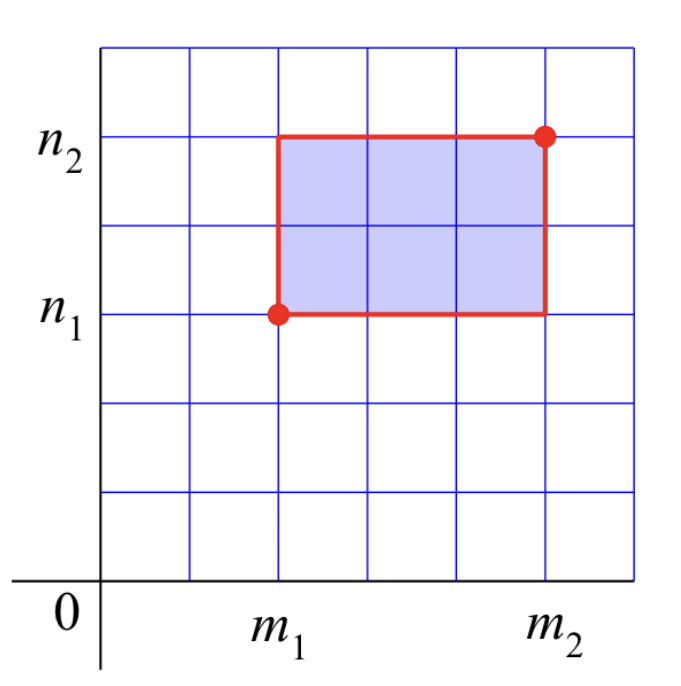
\includegraphics[scale=0.2]{Picture51.png}
\caption{An illiustration of the relative positions of $(m_1,n_1)$ and $(m_2, n_2)$ when $m_2>m_1$ and $n_2>n_1$.\fa}\label{figure51}
\end{figure}

 \begin{example}{}
The double sequence $\{a_{m,n}\}_{m,n=1}^{\infty}$ with
\[a_{m,n}=\frac{mn}{(m+1)(n+1)}\] is increasing in both indices.
\end{example}

The following is a counterpart of monotone convergence theorem for double sequences. 
 
\begin{theorem}[label=230301_11]
{Convergence of Increasing Double Sequences}
Let $\{a_{m,n}\}_{m,n=1}^{\infty}$ be a double sequence that is increasing in both indices. Then the double sequence $\{a_{m,n}\}_{m,n=1}^{\infty}$ is convergent if and only if it is bounded above. In case it is convergent, it converges to $\di\sup_{(m,n)\in\mathbb{Z}^+\times\mathbb{Z}^+}\{a_{m,n}\}$.
\end{theorem}
\begin{myproof}{Proof}
If the sequence $\{a_{m,n}\}_{m,n=1}^{\infty}$ converges to $a$, then there is a positive integer $N$ such that for all $(m,n)\in\mathbb{Z}^+\times\mathbb{Z}^+$ with $m\geq N$ and $n\geq N$, 
\[|a_{m,n}-a|<1.\]
This implies that 
\[a_{m,n}<a+1 \quad \text{ for all }\; m\geq N, n\geq N.\]Given $(m,n)\in\mathbb{Z}^+\times \mathbb{Z}^+$, let $k=\max\{m,n,N\}$. Then $k\geq m$, $k \geq n$ and $k\geq N$. Therefore,
\[a_{m,n}\leq  a_{k,k}<a+1.\]\bp
This prove  that the double sequence $\{a_{m,n}\}_{m,n=1}^{\infty}$ is bounded above by $a+1$.
In fact, the same reasoning shows that it is bounded above by $a+\varepsilon$ for any $\varepsilon>0$, but we do not need this.
 
Conversely, if $\{a_{m,n}\}_{m,n=1}^{\infty}$ is bounded above, then 
\[a=\sup_{(m,n)\in\mathbb{Z}^+\times\mathbb{Z}^+}\{a_{m,n}\}\]  exists. Given $\varepsilon>0$, there exists $(m_0, n_0)\in\mathbb{Z}^+\times \mathbb{Z}^+$ such that 
\[a_{m_0,n_0}>a-\varepsilon.\]
 Take $N=\max\{m_0,n_0\}$. Then if $m\geq N\geq m_0$, $n\geq N\geq n_0$,
\[a_{m,n}\geq   a_{m_0,n_0}> a-\varepsilon.\]
By definition $a_{m,n}\leq a$. Therefore, for all $(m,n)\in\mathbb{Z}^+\times\mathbb{Z}^+$ with $m\geq N$ and $n\geq N$, we have
\[|a_{m,n}-a|<\varepsilon.\]This proves that the double sequence $\{a_{m,n}\}_{m,n=1}^{\infty}$ is convergent and it converges to $\di a=\sup_{(m,n)\in\mathbb{Z}^+\times\mathbb{Z}^+}\{a_{m,n}\}$.
\end{myproof}

Now we turn to double series. A double series is a series of the form
\[\sum_{(m,n)\in\mathbb{Z}^+\times\mathbb{Z}^+}a_{m,n},\]where  $\{a_{m,n}\}_{m,n=1}^{\infty}$  is a double sequence. For each $(m,n)\in \mathbb{Z}^+\times\mathbb{Z}^+$, we define the $(m,n)$ partial sum $s_{m,n}$ by
\[s_{m,n}=\sum_{k=1}^m\sum_{l=1}^na_{k,l}.\]

\begin{definition}{Convergence of Double Series}
We say that the double series $\di\sum_{(m,n)\in\mathbb{Z}^+\times\mathbb{Z}^+}a_{m,n}$ is convergent provided that the double sequence of partial sums $\{s_{m,n}\}$ is convergent. In this case, the sum of the double series is
\[\sum_{(m,n)\in\mathbb{Z}^+\times\mathbb{Z}^+}a_{m,n}=s=\lim_{m,n\to\infty}s_{m,n}=\lim_{m,n\to\infty}\sum_{k=1}^m\sum_{l=1}^na_{k,l}.\]
\end{definition}

Notice that for any $(m,n)\in\mathbb{Z}^+\times \mathbb{Z}^+$,
\[s_{m,n}-s_{m,n-1}=\sum_{k=1}^m a_{k,n}.\]
Therefore,
\[s_{m,n}-s_{m,n-1}-s_{m-1,n}+s_{m-1, n-1}=\sum_{k=1}^ma_{k,n}-\sum_{k=1}^{m-1}a_{k,n}=a_{m,n}.\]
From this, we obtain the following immediately.

\begin{proposition}{}
If the double series $\di \sum_{(m,n)\in\mathbb{Z}^+\times\mathbb{Z}^+}a_{m,n}$ is convergent, then the double sequence   $\{a_{m,n}\}_{m,n=1}^{\infty}$  converges to 0.
\end{proposition}
 
\begin{figure}[ht]
\centering
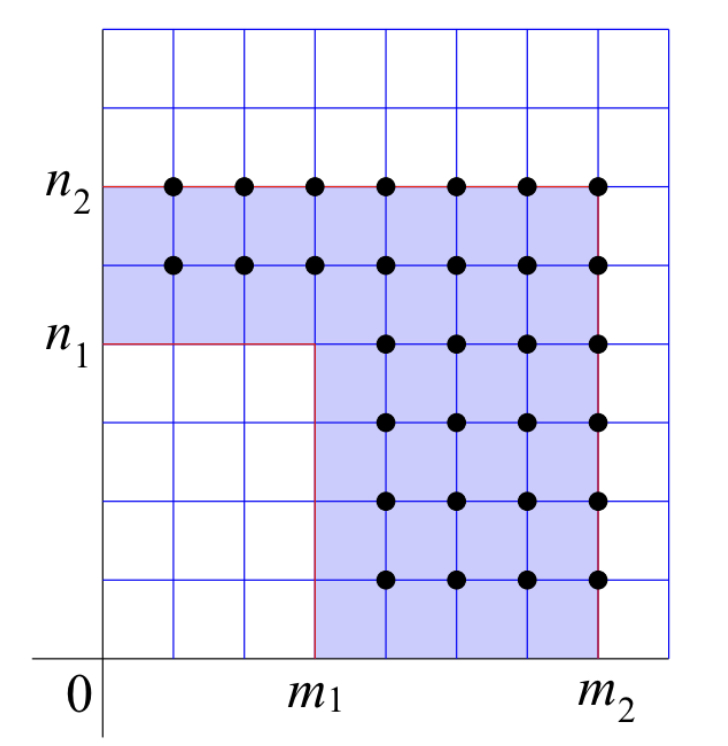
\includegraphics[scale=0.2]{Picture49.png}
\caption{An illiustration of those terms $a_{k,l}$  that involved in $s_{m_2, n_2}- s_{m_1, n_1}$ when $m_2>m_1$ and $n_2>n_1$.\fa}\label{figure49}
\end{figure}

If $\di\sum_{(m,n)\in\mathbb{Z}^+\times\mathbb{Z}^+}a_{m,n}$ is a double series with $a_{m,n}\geq 0$ for all $(m,n)\in\mathbb{Z}^+\times\mathbb{Z}^+$, then the double sequence of partial sums $\{s_{m,n}\}$ is a double sequence that is increasing in both indices.
From Theorem \ref{230301_11}, we obtain the following.
\begin{theorem}[label=230302_2]{}
If $\di\sum_{(m,n)\in\mathbb{Z}^+\times\mathbb{Z}^+}a_{m,n}$ is a double series with $a_{m,n}\geq 0$ for all $(m,n)\in\mathbb{Z}^+\times\mathbb{Z}^+$, then it is convergent if and only if the double sequence of partial sums $\{s_{m,n}\}$ is bounded above.
\end{theorem}
\begin{corollary}[label=230302_16]{}
If $\di\sum_{(m,n)\in\mathbb{Z}^+\times\mathbb{Z}^+}a_{m,n}$ is a double series with $a_{m,n}\geq 0$ for all $(m,n)\in\mathbb{Z}^+\times\mathbb{Z}^+$, then it is convergent if and only if the  sequence   $\{s_{n,n}\}_{n=1}^{\infty}$ is convergent. In this case,
\[\sum_{(m,n)\in\mathbb{Z}^+\times\mathbb{Z}^+}a_{m,n}=\lim_{n\to\infty}s_{n,n}=\lim_{n\to\infty}\sum_{k=1}^n\sum_{l=1}^na_{k,l}.\]
\end{corollary}
This says that we can determine the convergence of a nonnegative double series from the sequence $\{s_{n,n}\}_{n=1}^{\infty}$ instead of the double sequence $\{s_{m,n}\}_{m,n=1}^{\infty}$.
\begin{myproof}{Proof}Since $a_{m,n}\geq 0$ for all $(m,n)\in\mathbb{Z}^+\times\mathbb{Z}^+$, the double sequence $\{s_{m,n}\}$ is increasing in both indices, while the sequence $\{s_{n,n}\}$ is increasing.

If the double series $\di\sum_{(m,n)\in\mathbb{Z}^+\times\mathbb{Z}^+}a_{m,n}$ is convergent, Theorem \ref{230302_2} implies that the double sequence of partial sums $\{s_{m,n}\}$ is bounded above. Being a subset, the sequence   $\{s_{n,n}\}_{n=1}^{\infty}$ is also bounded above. By monotone convergence theorem,  the  sequence   $\{s_{n,n}\}_{n=1}^{\infty}$ is convergent. 
\bp
Conversely, assume that  the  sequence   $\{s_{n,n}\}_{n=1}^{\infty}$ is convergent. Then it is bounded above. Let \[t=\sup_{n\in\mathbb{Z}^+}s_{n,n}=\lim_{n\to\infty}s_{n,n}.\]For any positive integers $m$ and $n$, \[s_{m,n}\leq\max\{s_{m,m},s_{n,n}\}\leq t.\]
This implies that the double sequence   $\{s_{m,n}\}$ is bounded above by $t$. Hence, the double series $\di\sum_{(m,n)\in\mathbb{Z}^+\times\mathbb{Z}^+}a_{m,n}$ is convergent.  From the argument above, we also find that
\[\sup_{(m,n)\in\mathbb{Z}^+\times\mathbb{Z}^+}s_{m,n}\leq t=\sup_{n\in\mathbb{Z}^+}s_{n,n}.\]
Since the oppositie inequality is obvious, this is in fact an equality. Hence,
\begin{align*}\sum_{(m,n)\in\mathbb{Z}^+\times\mathbb{Z}^+}a_{m,n}&=\sup_{(m,n)\in\mathbb{Z}^+\times\mathbb{Z}^+}s_{m,n}=\sup_{n\in\mathbb{Z}^+}s_{n,n}\\&=\lim_{n\to\infty}s_{n,n}=\lim_{n\to\infty}\sum_{k=1}^n\sum_{l=1}^na_{k,l}.\end{align*}
\end{myproof}

Let us look at an example.
\begin{example}{}
Show that the double series
\[\sum_{(m,n)\in\mathbb{Z}^+\times\mathbb{Z}^+}\frac{1}{(m^2+n^2)^2}\] is convergent.
\end{example}
\begin{solution}{Solution}
Notice that 
\begin{align*}
s_{n,n}&=\sum_{k=1}^n\sum_{l=1}^n\frac{1}{(k^2+l^2)^2} \leq  \sum_{k=1}^n\sum_{l=1}^k \frac{1}{(k^2+l^2)^2}+\sum_{l=1}^n\sum_{k=1}^l \frac{1}{(k^2+l^2)^2}\\&
\leq 2\sum_{k=1}^n \sum_{l=1}^k\frac{1}{k^4} 
=2\sum_{k=1}^n\frac{k}{k^4}= 2\di\sum_{k=1}^{\infty}\frac{1}{k^3}.
\end{align*}Since the series $\di\sum_{k=1}^{\infty}\frac{1}{k^3}$ is convergent,     the sequence $\{s_{n,n}\}$ is bounded above. Hence,   the double series $\di\sum_{(m,n)\in\mathbb{Z}^+\times\mathbb{Z}^+}\frac{1}{(m^2+n^2)^2}$ is convergent.
\end{solution}



Next, we consider double series that have negative terms. 
Given a double sequence $\{a_{m,n}\}_{m,n=1}^{\infty}$, let $\{p_{m,n}\}_{m,n=1}^{\infty}$ and $\{q_{m,n}\}_{m,n=1}^{\infty}$ be double sequences defined by
\[p_{m,n}=\frac{|a_{m,n}|+a_{m,n}}{2},\hspace{1cm}q_{m,n}=\frac{|a_{m,n}|-a_{m,n}}{2}.\]Then
\[|a_{m,n}|=p_{m,n}+q_{m,n},\hspace{1cm}a_{m,n}=p_{m,n}-q_{m,n}.\]
 $\{p_{m,n}\}_{m,n=1}^{\infty}$ and $\{q_{m,n}\}_{m,n=1}^{\infty}$ are nonnegative double sequences with
\[0\leq p_{m,n}\leq |a_{m,n}|,\hspace{1cm}0\leq q_{m,n}\leq |a_{m,n}|.\]

 

\begin{definition}{Absolute Convergence of Double Series}We say that the double series $\di \sum_{(m,n)\in\mathbb{Z}^+\times\mathbb{Z}^+}a_{m,n}$
converges absolutely if the double series  $\di \sum_{(m,n)\in\mathbb{Z}^+\times\mathbb{Z}^+}|a_{m,n}|$ is convergent.
\end{definition}
\begin{theorem}[label=230302_12]{}
If the double series $\di \sum_{(m,n)\in\mathbb{Z}^+\times\mathbb{Z}^+}a_{m,n}$ converges absolutely, then it is convergent.
\end{theorem}
\begin{myproof}{Proof}
 For $(m,n)\in\mathbb{Z}^+\times\mathbb{Z}^+$, let
\[p_{m,n}=\frac{|a_{m,n}|+a_{m,n}}{2},\hspace{1cm}q_{m,n}=\frac{|a_{m,n}|-a_{m,n}}{2}.\]Then \[0\leq p_{m,n}\leq |a_{m,n}|,\hspace{1cm}0\leq q_{m,n}\leq |a_{m,n}|.\]Let 
$\{s^+_{m,n}\}$, $\{s^-_{m,n}\}$, $\{t_{m,n}\}$ and $\{s_{m,n}\}$ be respectively the double sequences of partial sums for the double series $\di\sum_{(m,n)\in\mathbb{Z}^+\times\mathbb{Z}^+}p_{m,n}$, $\di\sum_{(m,n)\in\mathbb{Z}^+\times\mathbb{Z}^+}q_{m,n}$, $\di\sum_{(m,n)\in\mathbb{Z}^+\times\mathbb{Z}^+}|a_{m,n}|$ and $\di\sum_{(m,n)\in\mathbb{Z}^+\times\mathbb{Z}^+}a_{m,n}$. Then
\[t_{m,n}=s^+_{m,n}+s^-_{m,n},\hspace{1cm} s_{m,n}=s^+_{m,n}-s^-_{m,n}.\]Moreover,
\begin{equation}\label{eq230302_4}0\leq s^+_{m,n}\leq t_{m,n},\hspace{1cm}0\leq s^-_{m,n}\leq t_{m,n}.\end{equation}
Since $\{p_{m,n}\}$, $\{q_{m,n}\}$ and $\{|a_{m,n}|\}$ are nonnegative double sequences, $\{s^+_{m,n}\}$, $\{s^-_{m,n}\}$ and $\{t_{m,n}\}$ are nonnegative double sequences that are increasing in both indices. By assumption, the double series $\di \sum_{(m,n)\in\mathbb{Z}^+\times\mathbb{Z}^+}|a_{m,n}|$ is convergent. Therefore, the double sequence $\{t_{m,n}\}$ is bounded above. Eq. \eqref{eq230302_4} implies that the double sequences  $\{s^+_{m,n}\}$ and  $\{s^-_{m,n}\}$ are also bounded above. Hence, the   double sequences  $\{s^+_{m,n}\}$ and  $\{s^-_{m,n}\}$ are convergent. By linearity, the double sequence $\{s_{m,n}\}$ is also convergent and
\[\lim_{m,n\to\infty}s_{m,n}=\lim_{m,n\to\infty}s^+_{m,n}-\lim_{m,n\to\infty}s^-_{m,n}.\] This proves that the double series $\di \sum_{(m,n)\in\mathbb{Z}^+\times\mathbb{Z}^+}a_{m,n}$ is convergent, and
\[\sum_{(m,n)\in\mathbb{Z}^+\times\mathbb{Z}^+}a_{m,n}=\sum_{(m,n)\in\mathbb{Z}^+\times\mathbb{Z}^+}p_{m,n}-\sum_{(m,n)\in\mathbb{Z}^+\times\mathbb{Z}^+}q_{m,n}.\]
\end{myproof}There is a simpler proof of this theorem using the same idea as we prove the case for single series. The ideas in the proof that we present above have been used when we prove that any rearrangement of an absolutely convergent single series is convergent and has the same sum. It is a useful technique  for dealing with absolutely convergent series. One should compare this proof to the proof of Theorem \ref{230224_8} for convergence of improper integrals. In fact, infinite series and improper integrals are closely related. An improper integral $\di\int_{-\infty}^{\infty} f(x)dx$ is convergent if and only if the double limit
\[\lim_{a\to-\infty, b\to\infty}\int_a^bf(x)dx\] exists. This can be rephrased as for any two sequences $\{a_m\}$ and $\{b_n\}$ satisfying   $\di\lim_{m\to\infty}a_m=-\infty$ and $\di\lim_{n\to \infty}b_n=\infty$, the double sequence $\{F_{m,n}\}$, with 
\[F_{m,n}=\int_{a_m}^{b_n}f(x)dx\] is convergent and has the same limit.

As we have seen before, we cannot simply compute the limit of a double sequence by taking the limit with respect to one index first before the other. For double series, we cannot find the sum simply by taking the sum with respect to one index first before the other. Let us look at the following example.
\begin{example}[label=ex230301_6]{}
For $(m,n)\in\mathbb{Z}^+\times\mathbb{Z}^+$, let
\[a_{m,n}=\begin{cases} m-n, \quad &\text{if}\;|m-n|=1,\\0,\quad &\text{otherwise},\end{cases}\] and consider the double series $\di\sum_{(m,n)\in\mathbb{Z}^+\times\mathbb{Z}^+}a_{m,n}$. We find that
\begin{align*}
\sum_{n=1}^{\infty}a_{m,n}=\begin{cases}-1,\quad &\text{if} \; m=1,\\0,\quad &\text{if}\;m\geq 2;\end{cases}\hspace{1cm} \sum_{m=1}^{\infty}a_{m,n}=\begin{cases}1,\quad &\text{if} \; n=1,\\0,\quad &\text{if}\;n\geq 2.\end{cases}
\end{align*}\be Therefore,
\[\sum_{m=1}^{\infty}\left(\sum_{n=1}^{\infty}a_{m,n}\right)=-1,\hspace{1cm}\sum_{n=1}^{\infty}\left(\sum_{m=1}^{\infty}a_{m,n}\right)=1.\]We find that changing the orders of summation produces different sums.
\end{example2}

\begin{figure}[ht]
\centering
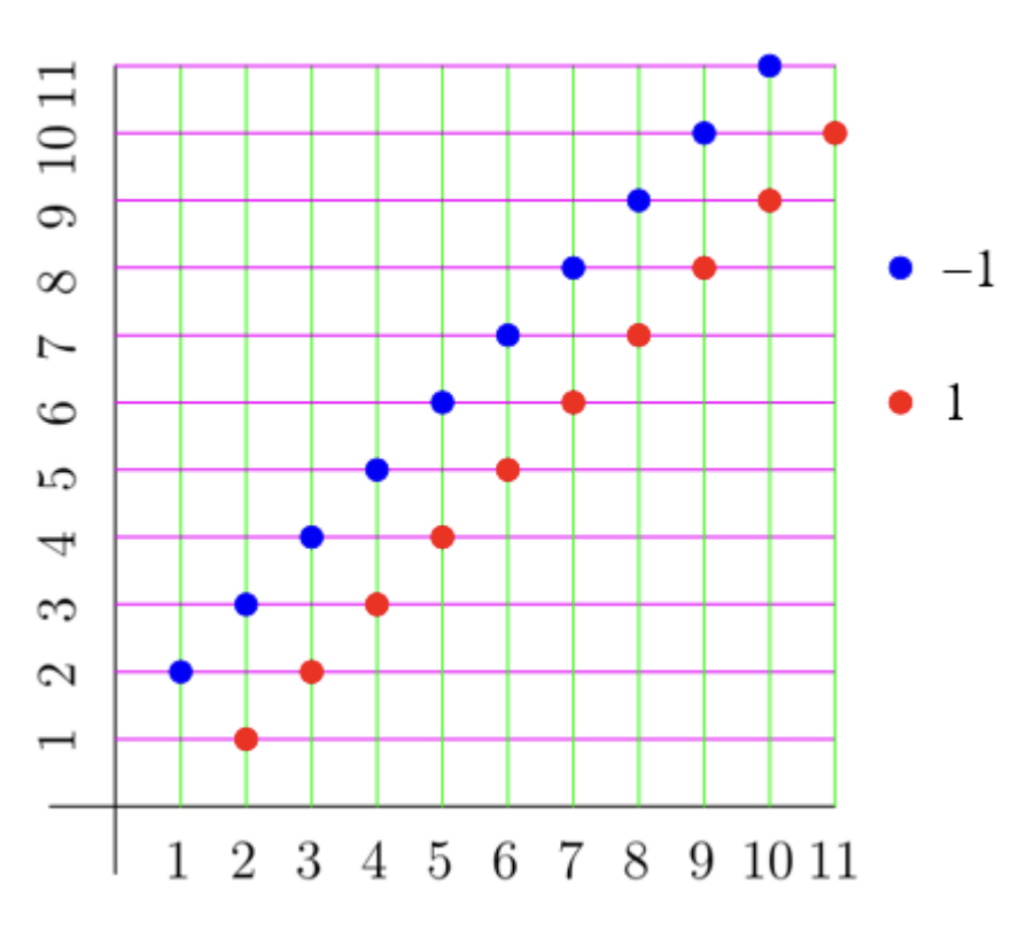
\includegraphics[scale=0.2]{Picture50.png}
\caption{An illiustration of the terms in the double series defined in Example \ref{ex230301_6}.\fa}\label{figure50}
\end{figure}

However, we have the following if the double series is convergent.
\begin{theorem}[label=230302_8]
{}
Assume that the double series $\di\sum_{(m,n)\in\mathbb{Z}^+\times\mathbb{Z}^+}a_{m,n}$ converges to $s$, and for every fixed $m\in\mathbb{Z}^+$, the series
$\di\sum_{n=1}^{\infty}a_{m,n}$ is convergent with sum $u_m$. Then the series \[\sum_{m=1}^{\infty}u_m=\sum_{m=1}^{\infty}\left(\sum_{n=1}^{\infty}a_{m,n}\right)\] is convergent and its sum is $s$.
\end{theorem}
\begin{myproof}{Proof}
  Let 
\[s_{m,n}=\sum_{k=1}^m\sum_{l=1}^na_{k,l}.\]  We are given that the double sequence $\{s_{m,n}\}_{m,n=1}^{\infty}$ converges to $s$. Notice that for fixed $m\in\mathbb{Z}^+$,
\[\sum_{k=1}^m u_k=\sum_{k=1}^m \lim_{n\to\infty}\sum_{l=1}^na_{k,l} =\lim_{n\to\infty}s_{m,n}.\] This shows that for fixed $m$, the limit $\di b_m= \lim_{n\to\infty}s_{m,n} $ exists and it equal to $\di\sum_{k=1}^m u_k$.
By Theorem \ref{230301_10}, the sequence $\{b_m\}$ converges to $s$. Therefore, the series $\di\sum_{m=1}^{\infty}u_m$ is convergent and has sum $s$.
\end{myproof}

Let us explore more about
  nonnegative double series first.

\begin{theorem}[label=230302_6]{}
Given that $\di\sum_{(m,n)\in\mathbb{Z}^+\times\mathbb{Z}^+}a_{m,n}$ is a double series with $a_{m,n}\geq 0$ for all $(m,n)\in\mathbb{Z}^+\times\mathbb{Z}^+$, and 
it is convergent with sum $s$.  We have the following.
\begin{enumerate}[(a)]
\item For all $m\in\mathbb{Z}^+$, $\di u_m=\sum_{n=1}^{\infty}a_{m,n}$ is finite.
\item For all $n\in\mathbb{Z}^+$, $\di v_n=\sum_{m=1}^{\infty}a_{m,n}$ is finite.
\item The series $\di\sum_{m=1}^{\infty}u_m$ and the series $\di\sum_{n=1}^{\infty}v_n$ both converge to $s$. Namely,
\[\sum_{m=1}^{\infty} \sum_{n=1}^{\infty} a_{m,n} =\sum_{n=1}^{\infty} \sum_{m=1}^{\infty} a_{m,n}=\sum_{(m,n)\in\mathbb{Z}^+\times\mathbb{Z}^+}a_{m,n}.\]
 \end{enumerate}
\end{theorem}
\begin{myproof}{Proof}
Given positive integers $m$ and $n$, let
\[s_{m,n}=\sum_{k=1}^m\sum_{l=1}^na_{m,n},\quad u_{m,n}=\sum_{l=1}^n a_{m,l},\quad v_{m,n}=\sum_{k=1}^ma_{k,n}.\]Then 
\begin{equation}\label{eq230302_7}
s_{m,n}=\sum_{k=1}^mu_{k,n}=\sum_{l=1}^n v_{m,l}.\end{equation}Since $a_{m,n}\geq 0$ for all $m, n\in\mathbb{Z}^+$, we have
\[u_{m,n}\leq s_{m,n},\hspace{1cm}v_{m,n}\leq s_{m,n}\hspace{1cm}\text{for all}\;(m,n)\in\mathbb{Z}^+\times\mathbb{Z}^+.\]
For fixed $m$, $\{u_{m,n}\}_{n=1}^{\infty}$ and  $\{s_{m,n}\}_{n=1}^{\infty}$ are increasing sequences. For fixed $n$, $\{v_{m,n}\}_{m=1}^{\infty}$  and  $\{s_{m,n}\}_{m=1}^{\infty}$ are  increasing sequences.  

Since the double series $\di\sum_{(m,n)\in\mathbb{Z}^+\times\mathbb{Z}^+}a_{m,n}$ is convergent with sum $s$, $s_{m,n}\leq s$ for all positive integers $m$ and $n$. Therefore,
the sequences $\{u_{m,n}\}_{n=1}^{\infty}$, $\{s_{m,n}\}_{m=1}^{\infty}$, $\{v_{m,n}\}_{m=1}^{\infty}$ and $\{s_{m,n}\}_{m=1}^{\infty}$ are increasing sequences that are bounded above by $s$. 
Therefore, each of these sequences is convergent.  The convergence of the sequences $\{u_{m,n}\}_{n=1}^{\infty}$ and $\{v_{m,n}\}_{m=1}^{\infty}$ are precisely the statements in (a) and (b). By definition,
 \[u_m=\sum_{n=1}^{\infty}a_{m,n}=\lim_{n\to\infty}u_{m,n},\hspace{1cm}v_n=\sum_{m=1}^{\infty}a_{m,n}=\lim_{m\to\infty}v_{m,n}.\]
Now let
\[b_m=\sum_{k=1}^mu_k \hspace{1cm}\text{and}\hspace{1cm}c_n=\sum_{l=1}^nv_l\] be the partial sums of the series $\di\sum_{m=1}^{\infty}u_m$ and $\di\sum_{n=1}^{\infty}v_n$. 
From \eqref{eq230302_7}, we find that
\[\lim_{n\to\infty}s_{m,n}=\sum_{k=1}^mu_k=b_m,\hspace{1cm}\lim_{m\to\infty}s_{m,n}=\sum_{l=1}^nv_l=c_n.\]From these, we find that the sequences $\{b_m\}$ and $\{c_n\}$ are also increasing sequences that are bounded above by $s$.\bp Therefore, 
\[b=\lim_{m\to\infty}b_m\hspace{1cm}\text{and}\hspace{1cm}c=\lim_{n\to\infty}c_n\] exist, and $b\leq s$, $c\leq s$. We are now left to prove that $b=c=s$. It is sufficient to prove that $b=s$. Then $c=s$ follows by interchanging the roles of $m$ and $n$.
Given $\varepsilon>0$, using the fact that $s=\sup\di\left\{s_{n,n}\,|\,n\in\mathbb{Z}^+\right\}$ from Corollary \ref{230302_16}, we find that there is a positive integer $N$ such that
\[s_{N,N}>s-\varepsilon.\]But then
\[s_{N,N}=\sum_{m=1}^N\sum_{n=1}^Na_{m,n}\leq \sum_{m=1}^N\sum_{n=1}^{\infty}a_{m,n}=b_N.\]This shows that
\[b_N>s-\varepsilon.\]
Hence,
\[b=\sup_m b_m> s-\varepsilon.\] Since $\varepsilon>0$ is arbitrary, we conclude that $b\geq s$. Together with $b\leq s$ that is proved earlier, we conclude that $b=s$.

\end{myproof}


\begin{theorem}[label=230302_3]{}
Given that $\di\sum_{(m,n)\in\mathbb{Z}^+\times\mathbb{Z}^+}a_{m,n}$ is a double series with $a_{m,n}\geq 0$ for all $(m,n)\in\mathbb{Z}^+\times\mathbb{Z}^+$.
Assume that for each $m\in\mathbb{Z}^+$, the series $\di\sum_{n=1}^{\infty}a_{m,n}$ converges to $u_m$. If the series
$\di\sum_{m=1}^{\infty}u_m$ is convergent, then the double series $\di\sum_{(m,n)\in\mathbb{Z}^+\times\mathbb{Z}^+}a_{m,n}$ is convergent, and 
\[\sum_{(m,n)\in\mathbb{Z}^+\times\mathbb{Z}^+}a_{m,n}=\sum_{m=1}^{\infty}u_m=\sum_{m=1}^{\infty}\left( \sum_{n=1}^{\infty} a_{m,n}\right).\]

\end{theorem}
\begin{myproof}{Proof}
It is sufficient to prove that the convergence of the series
$\di\sum_{m=1}^{\infty}u_m$ implies the convergence of the double series $\di\sum_{(m,n)\in\mathbb{Z}^+\times\mathbb{Z}^+}a_{m,n}$. The last statement then follows from Theorem \ref{230302_8}. Assume that the series
$\di\sum_{m=1}^{\infty}u_m$ converges to $u$. Using the same notations  as in the proof of Theorem \ref{230302_6}, we find 
that for each positive integer $m$, the sequence $\{u_{m,n}\}_{n=1}^{\infty}$ increases to $u_m$. From \eqref{eq230302_7}, we find  that for any positive integers $m$ and $n$, 
\[s_{m,n}\leq\sum_{k=1}^m u_k\leq u.\]This shows that the double sequence $\{s_{m,n}\}_{m,n=1}^{\infty}$ is bounded above, and hence it is convergent. Therefore,  the double series $\di\sum_{(m,n)\in\mathbb{Z}^+\times\mathbb{Z}^+}a_{m,n}$ is convergent. 

\end{myproof}
\begin{remark}{}
Putting together Theorem \ref{230302_6} and Theorem \ref{230302_3}, we conclude the following. Given a double series $\di\sum_{(m,n)\in\mathbb{Z}^+\times\mathbb{Z}^+}a_{m,n}$    with nonnegative terms $a_{m,n}$, we can determine its convergence and find its sum by first checking whether for each fixed $m$, the series $\di\sum_{n=1}^{\infty}a_{m,n}$ is convergent. If yes,  find the sum, call it as $u_m$, and check whether the series $\di\sum_{m=1}^{\infty}u_m$ is convergent. If yes, then the double series $\di\sum_{(m,n)\in\mathbb{Z}^+\times\mathbb{Z}^+}a_{m,n}$   is convergent and its sum is given by $\di\sum_{m=1}^{\infty}u_m$. Namely, the sum of the double series $\di\sum_{(m,n)\in\mathbb{Z}^+\times\mathbb{Z}^+}a_{m,n}$  can be obtained by iterated summation. \end{remark}
\begin{highlight}{} We can also start with the series $\di\sum_{m=1}^{\infty}a_{m,n}$ for each fixed $n$. This shows that for double series with nonnegative terms,   we can   interchange the orders of summation. In fact, with slightly more effort, one can prove that we can sum in any orders.

If for some integer $m$, the series $\di\sum_{n=1}^{\infty}a_{m,n}$ is divergent, then the double series $\di\sum_{(m,n)\in\mathbb{Z}^+\times\mathbb{Z}^+}a_{m,n}$   is divergent. Even if the series $\di\sum_{n=1}^{\infty}a_{m,n}$ is convergent for all positive integers $m$, the series $\di\sum_{m=1}^{\infty}u_m$ can still be divergent. In this latter case, the double series $\di\sum_{(m,n)\in\mathbb{Z}^+\times\mathbb{Z}^+}a_{m,n}$   is divergent. An example is given by the double series
\[\sum_{(m,n)\in\mathbb{Z}^+\times\mathbb{Z}^+}\frac{1}{m^2+n^2}.\]
For fixed positive integer $m$, comparison with the series $\di \sum_{n=1}^{\infty}\frac{1}{n^2}$ shows that the series $\di\sum_{n=1}^{\infty}\frac{1}{m^2+n^2}$ is convergent.
By integral test, we find that
\[u_m=\sum_{n=1}^{\infty}\frac{1}{m^2+n^2}\geq \int_0^{\infty}\frac{1}{m^2+x^2}dx-\frac{1}{m^2}=\frac{\pi}{2m}-\frac{1}{m^2}>0.\]Since the series $\di\sum_{m=1}^{\infty}\frac{1}{m}$ is divergent but the series  $\di \sum_{n=1}^{\infty}\frac{1}{m^2}$  is convergent, the series $\di \sum_{m=1}^{\infty}\left(\frac{\pi}{2m}-\frac{1}{m^2}\right)$ is divergent. Hence, the series $\di\sum_{m=1}^{\infty}u_m$ is divergent.
\end{highlight}

Finally, we can come back to series with negative terms.
From Theorem \ref{230302_6}, we have the following.
\begin{theorem}[label=230302_10]{}
Given that $\di\sum_{(m,n)\in\mathbb{Z}^+\times\mathbb{Z}^+}a_{m,n}$ is a double series that converges absolutely, and 
it is convergent with sum $s$.  We have the following.
\begin{enumerate}[(a)]
\item For all $m\in\mathbb{Z}^+$, $\di u_m=\sum_{n=1}^{\infty}a_{m,n}$ is finite.
\item For all $n\in\mathbb{Z}^+$, $\di v_n=\sum_{m=1}^{\infty}a_{m,n}$ is finite.
\item The series $\di\sum_{m=1}^{\infty}u_m$ and the series $\di\sum_{n=1}^{\infty}v_n$ both converge to $s$. Namely,
\[\sum_{m=1}^{\infty} \sum_{n=1}^{\infty} a_{m,n} =\sum_{n=1}^{\infty} \sum_{m=1}^{\infty} a_{m,n}=\sum_{(m,n)\in\mathbb{Z}^+\times\mathbb{Z}^+}a_{m,n}.\]
 \end{enumerate}
 
\end{theorem}
\begin{myproof}{Proof}
  Using the same notations as in the proof of Theorem \ref{230302_12}, since the double series $\di\sum_{(m,n)\in\mathbb{Z}^+\times\mathbb{Z}^+}|a_{m,n}|$ is convergent, the double series $\di\sum_{(m,n)\in\mathbb{Z}^+\times\mathbb{Z}^+}p_{m,n}$ and $\di\sum_{(m,n)\in\mathbb{Z}^+\times\mathbb{Z}^+}q_{m,n}$ are convergent. Applying Theorem \ref{230302_6} to the nonnegative series $\di\sum_{(m,n)\in\mathbb{Z}^+\times\mathbb{Z}^+}p_{m,n}$ and $\di\sum_{(m,n)\in\mathbb{Z}^+\times\mathbb{Z}^+}q_{m,n}$, we conclude that for all $m\in\mathbb{Z}^+$ and all $n\in\mathbb{Z}^+$, the series
$\di \sum_{n=1}^{\infty}p_{m,n}$, $\di \sum_{n=1}^{\infty}q_{m,n}$,  $\di\sum_{m=1}^{\infty}p_{m,n}$ and $\di\sum_{m=1}^{\infty}q_{m,n}$  are convergent.  Since
\[a_{m,n}=p_{m,n}-q_{m,n}\hspace{1cm}\text{for all}\;(m,n)\in\mathbb{Z}^+\times\mathbb{Z}^+,\]
we conclude that the series
$\di \sum_{n=1}^{\infty}a_{m,n}$ and the series $\di\sum_{m=1}^{\infty}a_{m,n}$ are convergent. The remaining assertions are concluded using the same arguments.
\end{myproof}
This theorem says that absolutely convergent double series enjoys almost the same privileges as the nonnegative double series.
 The following theorem gives a summary.
\begin{theorem}{}
Given that $\di\sum_{(m,n)\in\mathbb{Z}^+\times\mathbb{Z}^+}a_{m,n}$ is a double series that satisfies the following conditions.
\begin{enumerate}[(i)]
\item
For each fixed $m\in\mathbb{Z}^+$, the series $\di\sum_{n=1}^{\infty}|a_{m,n}|$ is convergent.
\item $\di \sum_{m=1}^{\infty}\sum_{n=1}^{\infty}|a_{m,n}|$ is convergent.
\end{enumerate}
 We have the following.
\begin{enumerate}[(a)]
\item The double series $\di\sum_{(m,n)\in\mathbb{Z}^+\times\mathbb{Z}^+}a_{m,n}$ converges absolutely.
\item For each fixed $n\in\mathbb{Z}^+$, the series $\di\sum_{m=1}^{\infty}a_{m,n}$  converges absolutely.
\item For each fixed $m\in\mathbb{Z}^+$, the series $\di\sum_{n=1}^{\infty}a_{m,n}$  converges absolutely.
\item Both the series  $\di \sum_{m=1}^{\infty}\left|\sum_{n=1}^{\infty} a_{m,n}\right|$ and $\di \sum_{n=1}^{\infty}\left|\sum_{m=1}^{\infty} a_{m,n}\right|$ are convergent.
\item The sum of the double series can be computed by iterated summation. Namely, 
\[\sum_{(m,n)\in\mathbb{Z}^+\times\mathbb{Z}^+}a_{m,n}=\sum_{m=1}^{\infty} \sum_{n=1}^{\infty} a_{m,n} =\sum_{n=1}^{\infty} \sum_{m=1}^{\infty} a_{m,n}.\]
\end{enumerate}
\end{theorem}
\begin{myproof}{Proof}
By Theorem \ref{230302_3}, (i) and (ii) implies that the double series  $\di\sum_{(m,n)\in\mathbb{Z}^+\times\mathbb{Z}^+}|a_{m,n}|$ is convergent, which gives (a). \bp By  Theorem \ref{230302_6}, (a) implies (b) and (c). Theorem \ref{230302_6} also implies that
the two series
\[  \sum_{m=1}^{\infty}\left(\sum_{n=1}^{\infty} |a_{m,n}|\right)\quad\text{and }\quad   \sum_{n=1}^{\infty}\left(\sum_{m=1}^{\infty} |a_{m,n}|\right)\]are convergent.
 Since
\[\left|\sum_{n=1}^{\infty} a_{m,n}\right|\leq \sum_{n=1}^{\infty}\left| a_{m,n}\right|,\hspace{1cm}\left|\sum_{m=1}^{\infty} a_{m,n}\right|\leq \sum_{m=1}^{\infty}\left|   a_{m,n}\right|,\]comparison test shows that  the series  $\di \sum_{m=1}^{\infty}\left|\sum_{n=1}^{\infty} a_{m,n}\right|$ and $\di \sum_{n=1}^{\infty}\left|\sum_{m=1}^{\infty} a_{m,n}\right|$ are convergent. This gives   (d). The statement (e) follows from (a) and Theorem \ref{230302_10}.
\end{myproof}

\vp
\noindent
{\bf \large Exercises  \thesection}
\setcounter{myquestion}{1}
 
\begin{question}{\themyquestion}
If $a$ and $b$ are positive constants,  show that the double series 
\[\sum_{(m,n)\in \mathbb{Z}^+\times\mathbb{Z}^+}\frac{1}{am^2+bn^2}\] is divergent.
\end{question}
\atc

\begin{question}{\themyquestion}
Given that $a$ and $b$ are positive constants,  $u$ and $v$ are   real numbers, and $\alpha$ is a number larger than 1. Show that the double series 
\[\sum_{(m,n)\in \mathbb{Z}^+\times\mathbb{Z}^+}\frac{\sin(mu+nv)}{(am^2+bn^2)^{\alpha}}\] is convergent.
\end{question}
